% Delete the MSc option if you are doing a PhD, or replace it with MPhil
% for a Master of Philosophy thesis
%
% The 12pt option is required by the 2001/02 thesis regulations
% Last update 15th August 2007: new Abstract format and Copyright Statement

% Replace MSc with PhD for PhD theses
% Remove the twoside option for single-sided printing
\documentclass[12pt,MSc,twoside]{muthesis_2020}
\bibliographystyle{abbrv}
\usepackage{listings,amsmath,amssymb,xcolor,graphicx,url,natbib}
\usepackage{amsthm}
\newtheorem{theorem}{Theorem}[chapter]
\newtheorem{lemma}{Lemma}[chapter]
\usepackage{booktabs}
\usepackage{subfigure}
\usepackage{cases}
\usepackage{bm}
\usepackage{array}

\begin{document}
\title{Dynamics of an Elastic Particle in Viscous Shear Flow}
\author{Hao Ye}
% Faculty of Life Sciences people should comment the next line out
\school{Mathematics}
\faculty{Science and Engineering}
\def\wordcount{11172}

% Uncomment the line below to suppress the `List of Tables' page (optional)
\tablespagefalse

% Uncomment the line below to suppress the `List of Figures' page (optional)
\figurespagefalse

% Uncomment the line below to use a customised Declaration statement
%\def\declaration{All the work in this thesis has been sourced from Google.}

\beforeabstract

Investigating the dynamics of an elastic particle in viscous flow has gained significant attention in recent years due to its wide-ranging applications in biology, materials science, and engineering. In this report, we study the behaviour of an elastic particle in shear flow at a low Reynolds number, with a particular focus on its equilibrium state. The classical approach to this problem is based on the concept of fluid-solid interaction. In this study, we use slender body theory to evaluate the fluid traction and Kirchhoff-Love beam theory to derive the governing equation for the elastic beam, coupling both to form the system. To generalise our research, we select the boomerang shape as the initial configuration for the inextensible elastic particle in the numerical study. The deformations of the particle are classified into four types based on their characteristics. We present the plots of steady orientation against the fluid-solid interaction coefficient and observe that, for particles with one relatively short arm, increasing the opening angle between the two arms leads to bifurcations in the curve, eventually splitting out separate closed loops.






%\afterabstract

% The next part is optional; however it is a good place to thank your
% supervisor and the people responsible for providing computer support ;-)
%\prefacesection{Acknowledgements}
%I would like to thank...

% The next line is NOT optional and MUST appear
\afterpreface


% Finally, you can start writing about all the new theorems you have proved
% and all the new results that you have discovered

\chapter{Introduction}
\section{Background}
Stokes flow provides a useful entry point for exploring the rheology of a particle in a dilute suspension. Typically, the movement of a particle is governed by its interaction with the background flow rather than with other particles. Hence, investigating the dynamics of a single particle in Stokes flow is a worthwhile endeavour. In Stokes flow, where the Reynolds number is exceedingly low, the particle motion is primarily governed by viscous forces, and the inertial effects are negligible. In such a circumstance, the shape of the particle becomes a key factor in determining its motion. In early research, Stokes \cite{stokes1851effect} investigated the sedimentation of a solid sphere in viscous flow in 1851 and found that the motion was purely vertical. Then, in 1876, Oberbeck \cite{oberbeck1876ueber} conducted a similar study on an ellipsoid and was the first to obtain a solution for an ellipsoid at any orientation relative to a uniform flow using the Stokes equations. In 1963, Brenner \cite{brenner1963stokes} showed the possibility of constructing objects that maintain a stable orientation while exhibiting a constant horizontal drift. Such objects could be either asymmetric or bodies of revolution, such as a straight rod. Subsequently, more complex shapes have been analysed, including rigid non-axisymmetric ellipsoids \cite{hinch1979rotation}, rigid curved nonchiral fibres \cite{wang2012flipping}, and rigid boomerang-shaped particles \cite{roggeveen2022motion}. In contrast, chiral particles exhibit different behaviour, continuously reorienting while sedimenting, resulting in spiral trajectories \cite{doi2005motion}. 

After considering rigid particles, flexible fibres, which are more common in nature and have a wide range of applications, are also important. They are particularly relevant to various biological transport processes, such as swimming of microorganisms \cite{lauga2009hydrodynamics} and the transport of subcellular structures, including nuclei, chromosomes, and organelles \cite{shelley2016dynamics}. In addition, they have extensive industrial applications. In the paper industry, the orientation and spatial distribution of fibres in flowing pulp must be meticulously managed \cite{yasuda2004experimental}, while in petroleum engineering, fibres are employed to improve proppant transport in fracturing fluids and prevent proppant backflow \cite{howard1995fiber}. Currently, research on flexible fibres made of elastic materials is more popular due to their complex interactions with fluid flows and potential applications in microfluidics, biological systems, and soft matter physics. In 2000, Shelley and Ueda \cite{shelley2000stokesian} investigated the dynamics of slender elastic fibres in a viscous fluid and first developed a numerical method based on the slender body approximation to simulate flexible filaments. In fact, there are many methods applied in this area, such as the bead-spring model or the immersed boundary method. However, the local slender body theory is the mainstay of this research area, giving a local primary relation between elastic and drag forces \cite{lindner2015elastic}. A recent paper by Liu et al. \cite{liu2024spectral}, which investigated the dynamics of elastica in shear flow with spectral analysis. This research used local slender body theory to analyse object's dynamics, coupled with the inextensible Euler-Bernoulli beam model to account for elastic forces. Such problems typically involve fluid-solid interaction (FSI), making this a common approach to addressing these issues by considering the hydrodynamical and elastic components simultaneously. This method has also been validated by several previous studies that combine theoretical analysis and experimental verification, such as \cite{tornberg2004simulating}, \cite{quennouz2015transport}, \cite{liu2018morphological}.

Slender-shaped particles are widely observed in nature and many industries. Various microorganisms, including Salmonella typhimurium \cite{lauga2009hydrodynamics}, Volvox carteri \cite{goldstein2015green}, Paramecium \cite{brennen1977fluid}, and mammalian sperm cells \cite{gaffney2011mammalian}, use slender appendages to propel themselves through viscous fluids. In chemical engineering, the slender structure of fibres is used in the production of fibre-reinforced composites, which demonstrate enhanced tensile strength and increased anisotropic thermal conductivity \cite{tekce2007effect}. The definition of a slender body requires that the object have a small aspect ratio, which is the ratio of the object's cross-sectional radius to its length. For objects with this characteristic immersed in Stokes flow, where inertia forces are negligible, slender body theory is a particularly appropriate analytical method. This theory was initiated by Burgers \cite{burgers1938motion} in $1938$, but did not attract much academic attention at the time. Several years later, in 1960, Broersma \cite{broersma1960rotational}\cite{broersma1960viscous} took note of this outcome and made a slight improvement to the original form of the theory. Subsequently, numerous scholars, including Tuck \cite{tuck1964some}\cite{tuck1970toward}, Taylor \cite{taylor1969motion}, Cox \cite{cox1970motion}\cite{cox1971motion}, and Tillett \cite{tillett1970axial}, have continued to study and refine the theory, ultimately leading to the more general form we see today. 

Typically, shear flow is very common, even ubiquitous, in applications where fibres experience flow. For instance, Poiseuille or Couette flows can be approximated as shear flows at sufficiently small scales. There are many studies on rigid body objects immersed in shear flow, which can be traced back to $1922$ when Jeffery \cite{jeffery1922motion} published his seminal work on the periodic tumbling motion of rigid ellipsoidal particles in shear flow, known as Jeffery orbits. This motion is parameterized only by the initial orientation of the particle relative to the flow. The orbital period is dependent on the aspect ratio of the particle. The equation governing the angular evolution is known as Jeffery's equation, and in 1962, Bretherton \cite{bretherton1962motion} expanded on this work, showing that this equation also applies to an arbitrary body of revolution. Expanding to elastic particles, a recent study demonstrates that initially straight slender elastic filaments deform in shear flow and display tumbling motions similar to Jeffery orbits, with orbital constants that either decrease or increase exponentially over time \cite{zuk2021universal}.

We are particularly interested in a paper published by Roggeveen and Stone \cite{roggeveen2022motion}. They studied the motion of asymmetric bodies in two-dimensional shear flow at a low Reynolds number, selecting a representative composite shape, the rigid boomerang, as their research object. Their motivation is clear: since most particles in nature are not symmetric, and numerous previous studies have demonstrated that reduced symmetry significantly impacts particle motion, they sought to investigate more realistic, asymmetric particles. According to a study by De Canio et al. \cite{de2017spontaneous}, the boomerang shape can qualitatively represent the behaviour of more complex bodies. Thus, boomerang-shaped particles are a highly suitable object for their research. 
This paper used two parameters to describe the shape of the rigid boomerang-shaped particle. The aspect ratio, $q$, defines the lengths of the particle's arms, while $\alpha$ represents the opening angle between the two arms. Figure \ref{fig:17} depicts the definition of the particle's geometry. 
\begin{figure}[htb]
	\begin{center}
		% specify width as 80% of the width of the text on the page
		% we can also specify a width in centimetres, e.g. [width=8cm]
		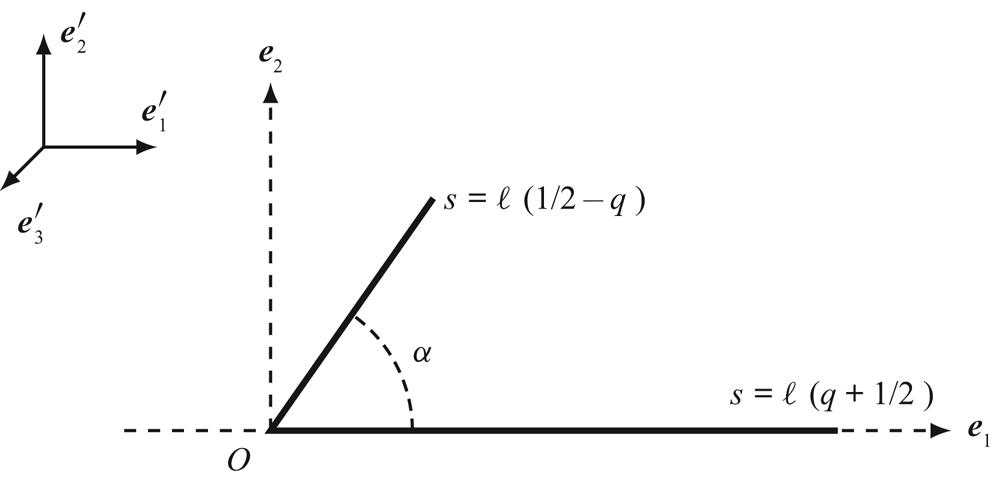
\includegraphics[width=0.7\textwidth]{plot/stone2.png}
		\caption{This is the plot from the Roggeveen and Stone's paper \cite{roggeveen2022motion}. The geometry of the rigid boomerang-shaped particle.}
    \label{fig:17}
	\end{center}
	%	\setlength{\abovecaptionskip}{-0.5 cm}
\end{figure}
This paper used the mobility and resistance matrices to relate the particle's translational velocity and rate of rotation to the forces and torques acting on it. In addition, they applied slender body theory to evaluate the traction exerted by the fluid on the particle. They demonstrated that a general force-free and torque-free particle placed in the plane of a two-dimensional shear flow will exhibit one of two possible behaviours: periodic cross-streamline motion while tumbling or persistent cross-streamline drift at a fixed angle. Specifically, there are four fixed orientations $\theta_0$ for a given particle shape, and of the four solutions, two differ from the other two by an angle of $\pi$, as shown in Figure \ref{fig:18}. Two solutions differing by $\pi$ are either stable or unstable.
\begin{figure}[htb]
	\begin{center}
		% specify width as 80% of the width of the text on the page
		% we can also specify a width in centimetres, e.g. [width=8cm]
		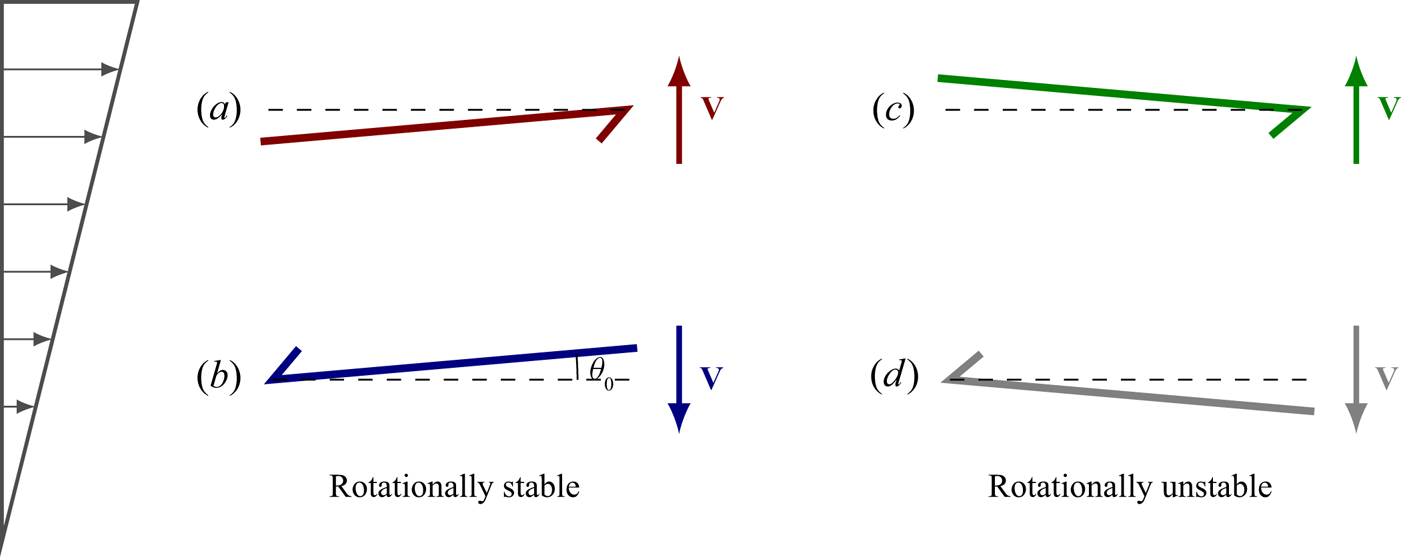
\includegraphics[width=1\textwidth]{plot/stone3.png}
		\caption{This is the plot from the Roggeveen and Stone's paper \cite{roggeveen2022motion}. Illustrative fixed orientations with $q=0.4$ and $\alpha=\frac{\pi}{4}$ shown relative to the background shear flow. The orientation angle for this shape, $\theta_0\approx0.038$, has been exaggerated here for clarity.}
    \label{fig:18}
	\end{center}
	%	\setlength{\abovecaptionskip}{-0.5 cm}
\end{figure}
Next, they present a $q-\alpha$ plot to demonstrate the types of shapes that can maintain a fixed orientation in shear flow, as illustrated in Figure \ref{fig:19}. Note that the aspect ratio $q$ and the opening angle $\alpha$ are the only two parameters defining the particle's geometry. In the grey region, the particle will adopt a fixed orientation relative to the flow and drift across streamlines. This behaviour is observed exclusively in shapes with significant asymmetry and a relatively small opening angle $\alpha$. Beyond this region, the particles undergo continuous rotation, exhibiting periodic motion with respect to the surrounding flow.
\begin{figure}[htb]
	\begin{center}
		% specify width as 80% of the width of the text on the page
		% we can also specify a width in centimetres, e.g. [width=8cm]
		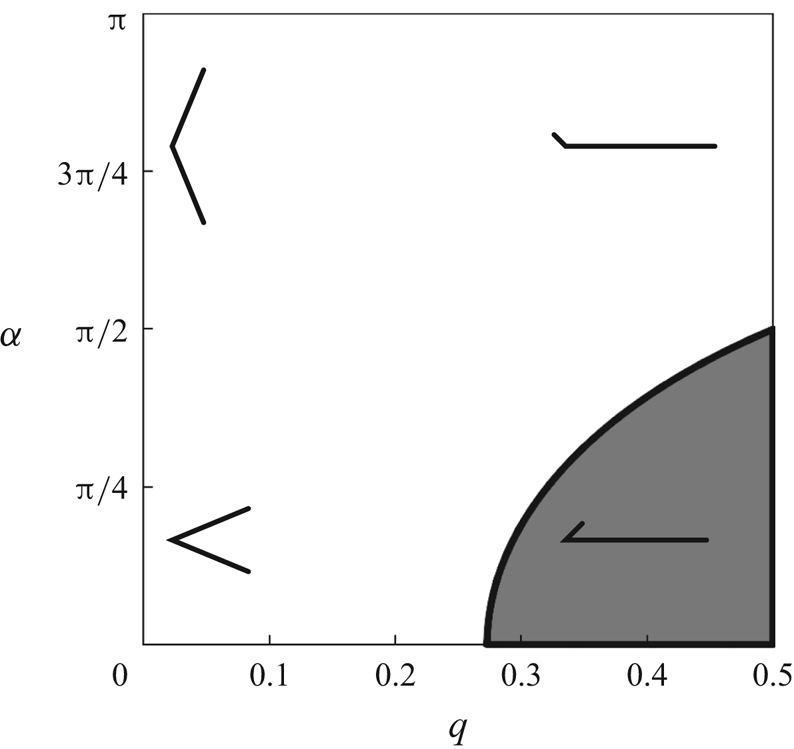
\includegraphics[width=0.6\textwidth]{plot/stone.png}
		\caption{This is the plot from the Roggeveen and Stone's paper \cite{roggeveen2022motion}. The grey region in $q-\alpha$ parameter space represents the bodies for which fixed points exist.}
    \label{fig:19}
	\end{center}
	%	\setlength{\abovecaptionskip}{-0.5 cm}
\end{figure}


Building on this study, we aim to investigate the behaviour of particles with the same shape but with inextensible elastic properties. More specifically, we intend to set the boomerang shape as the initial configuration of the elastic particle. Using the same fluid as in previous considerations, we will explore the dynamics of these elastic particles in shear flow at a low Reynolds number. More importantly, we anticipate observing the various deformations of the particle under these circumstances. This is crucial because understanding how the particle deforms in response to the fluid flow can provide insight into the underlying mechanisms governing its dynamics, which may have significant implications for applications such as designing advanced materials with tailored properties, optimising drug delivery systems in biomedical engineering, and enhancing the performance of microfluidic devices. To model this problem, we will adopt the classic approach involving the fluid-solid interaction (FSI). The general idea is that flow-induced stresses deform the object, and the deformed object then interacts hydrodynamically with nearby boundaries, which in turn alters the object's motion. This means that we cannot approach such problems with a simple cause-and-effect sequence. Since the particle's shape influences its motion, and the motion, in turn, affects its shape through fluid forces, the problem is inherently dynamic and must be tackled simultaneously. To quantify this, we will introduce a fluid-solid interaction coefficient, $\mathcal{I}$, which measures the degree or strength of interaction between the fluid and the solid within the system. Then, the results of the rigid particles from Roggeveen and Stone \cite{roggeveen2022motion} will serve as a special case in our project when the FSI coefficient $\mathcal{I}=0$. This makes it a valuable reference for validating our results.

\section{Slender body theory}
Here, we introduce the basic theory of slender body theory. Consider a rigid incompressible but perhaps flexible long slender body. We assume that the body has length $2L$ and a typical cross-sectional radius $a\ll L$. We define the aspect ratio $\epsilon=\frac{a}{L}\ll 1$. We assume that the radius only varies on the long length scale $L$ and any curvature of the centre-line is $O(L^{-1})$. Let the position of the centre-line of the body be given by $\mathbf{X}(s,t)$, where $s \in (-L,L)$ is arc-length and $t$ is time. We can define the tangent vector $\hat{\mathbf{t}}(s,t)$ to the centre-line and the velocity $\mathbf{V}(s,t)$ of the body in terms of $\mathbf{X}$ by
\begin{equation}
\label{eqn:105}
\hat{\mathbf{t}}=\frac{\partial \mathbf{X}}{\partial s}, \quad \mathbf{V}=\frac{\partial\mathbf{X}}{\partial t}.
\end{equation}
The background flow is given by $\mathbf{u}^\infty$. Then, the traction $\mathbf{f}$ (hydrodynamic force-density) exerted by the fluid is 
\begin{equation}
\label{eqn:106}
\mathbf{f}\sim \frac{4\pi\mu}{\log(\frac{1}{\epsilon})}\Bigg(\mathbf{I}-\frac{1}{2} \hat{\mathbf{t}}\hat{\mathbf{t}}\Bigg)\cdot(\mathbf{u}^\infty-\mathbf{V}),
\end{equation}
where $\mu$ denotes the uniform dynamic viscosity.
\section{Outline}
The following parts of the report are organized as follows.
In Chapter 2, we introduce the basic setup of this project, which includes the non-dimensional Stokes equations, reference frames and flow. Additionally, through derivation, we reduce this three-dimensional problem to two dimensions. Chapter 3 presents the theoretical framework of this project. We begin by introducing the fluid-solid interaction, the classical concept underlying this type of problem. We find that the deformation of the particle is time-independent and derive the specific expression for the translational vector. Subsequently, we establish the equilibrium equations for the system and implement them using the finite element method in conjunction with the Newton method. Chapter 4 focuses on the numerical results. We use \texttt{oomph-lib}\footnote{\texttt{oomph-lib} is an object-oriented, open-source finite-element library for the simulation of multi-physics problems.}, a C++-based library, to develop the algorithm and perform numerical computations. The elastic boomerang-shaped particle is selected as the research object, and the numerical data are visualised through various plots to illustrate the particle's deformation at different values of the FSI coefficient. In addition, we present plots of the steady orientation against the FSI coefficient, revealing some interesting bifurcations along the curve. A similar plot to Figure \ref{fig:19}, the $q-\alpha$ plot, is produced but for different values of the FSI coefficient. Lastly, we define the tensile stress for the rigid case to demonstrate the trend of deformation caused by fluid forces. Chapter 5 concludes the entire study, and Chapter 6 offers insight into future research directions.


\chapter{Basic Setup}

\section{Stokes equations}
Recall that the Navier–Stokes Equations for the flow of an incompressible Newtonian fluid with uniform density $\rho$ and uniform dynamic viscosity $\mu$ are 
\begin{equation}
\label{eqn:11}
\begin{aligned}
        \rho\frac{D\mathbf{u}^*}{Dt^*}&=-\bm{\nabla}^*p^*+\mu \nabla^{*2}\,\mathbf{u}^*,\\
        \bm{\nabla}^*\cdot \mathbf{u}^*&= 0,
\end{aligned}
\end{equation}
where $\mathbf{u}^*$ is the velocity field and $p$ is the pressure. Since our research object is a particle, we assume that there is no body force acting on it. We set the total length of the particle as the characteristic length $\mathcal{L}$ and define the time scale as $\frac{1}{\dot{\gamma}}$, where $\dot{\gamma}$ is the shear rate. This implies that the characteristic velocity is $\mathcal{U^*}=\mathcal{L}\dot{\gamma}$ and also simplifies the characteristic pressure on the associated viscous scale as $\frac{\mu \,\mathcal{U^*}}{\mathcal{L}}=\mu\dot{\gamma}$. Then, we use these scales to dimensionless the Navier-Stokes equations above, where the non-dimensional variables are denoted without asterisks. Substituting these scales and non-dimensional variables into \eqref{eqn:11}, we obtain 
\begin{equation}
\label{eqn:12}
\begin{aligned}
\rho\left(\mathcal{L}\dot{\gamma}^2\frac{\partial\mathbf{u}}{\partial t}+\mathcal{L}\dot{\gamma}^2\,\mathbf{u}\cdot\bm{\nabla}\mathbf{u} \right)&=-\frac{\mu\dot{\gamma}}{\mathcal{L}}\,\bm{\nabla} p+\frac{\mu\dot{\gamma}}{\mathcal{L}}\,\nabla^{2}\mathbf{u},\\
\dot{\gamma}\,\bm{\nabla}\cdot\mathbf{u}&=0.
\end{aligned}
\end{equation}
Hence, the non-dimensional Navier–Stokes Equations are given by
\begin{equation}
\label{eqn:13}
\begin{aligned}
\rho\left(\frac{\partial\mathbf{u}}{\partial t}+\mathbf{u}\cdot\bm{\nabla}\mathbf{u} \right)&=-\frac{\mu}{\mathcal{L}^2\dot{\gamma}}\,\bm{\nabla} p+\frac{\mu}{\mathcal{L}^2\dot{\gamma}}\,\nabla^{2}\mathbf{u},\\
\bm{\nabla}\cdot\mathbf{u}&=0.
\end{aligned}
\end{equation}
From \eqref{eqn:13}, we assume that the Reynolds number is 
\begin{equation}
\label{eqn:14}  
Re=\frac{\mathcal{L}^2\dot{\gamma}\rho}{\mu}.
\end{equation}
If $Re \ll 1$ then inertia is negligible relative to viscosity, and \eqref{eqn:13} can be approximated by 
\begin{equation}
\label{eqn:15}
\begin{aligned}
\bm{\nabla} p&=\nabla^{2}\mathbf{u},\\
\bm{\nabla}\cdot\mathbf{u}&=0,
\end{aligned}
\end{equation}
which are the non-dimensional Stokes equations. 





\section{Frames and flow}
We establish a reference frame fixed to the particle, with axes $\{\mathbf{e_1},\mathbf{e_2},\mathbf{e_3}\}$ suitably aligned with the particle's geometry relative to a designated origin $O$. As shown in Figure \ref{fig:3} (left), the particle-fixed reference frame $\{\mathbf{e_1},\mathbf{e_2},\mathbf{e_3}\}$ is attached to the elastic object, with its end point designated as the origin $O$. In addition, the circumstance we are concerned with for the research object is a shear flow $\dot{\gamma}$, shown in Figure \ref{fig:3} (right). We also define a laboratory reference frame $\{\mathbf{e'_1},\mathbf{e'_2},\mathbf{e'_3}\}$ for the shear flow, such that $\mathbf{e'_1}$ aligns with the direction of the streamlines, $\mathbf{e'_2}$ aligns with the direction of the flow gradient, and $\mathbf{e'_3}$ aligns with the direction of the vorticity. In this frame, the background flow is given by 
\begin{equation}
\label{eqn:104}
    \mathbf{U}^{\infty*}(\mathbf{x}^*)=\dot{\gamma}y^*\mathbf{e'_1},
\end{equation}
where $y^*$ is the second component of the position vector $\mathbf{x}^*$. 
\begin{figure}[htb]
	\begin{center}
		% specify width as 80% of the width of the text on the page
		% we can also specify a width in centimetres, e.g. [width=8cm]
		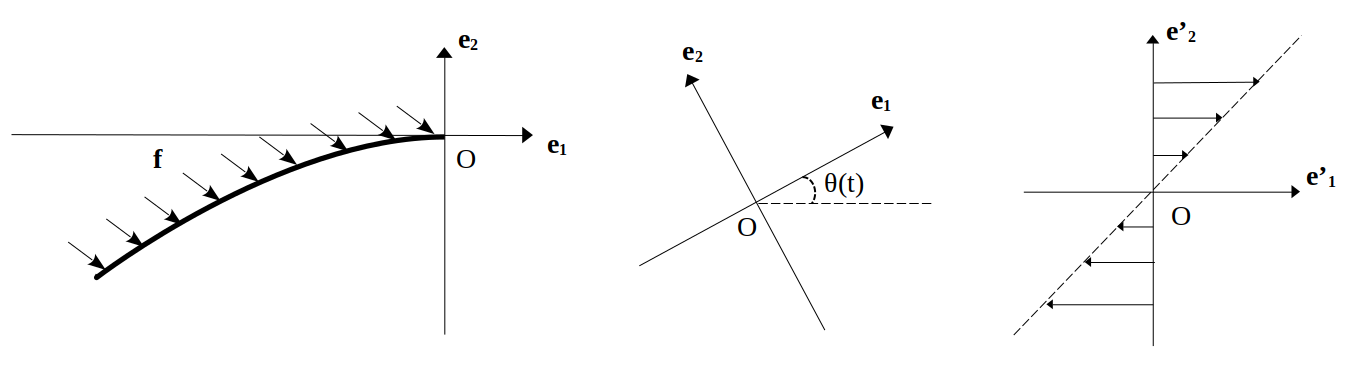
\includegraphics[width=1\textwidth]{plot/frames_general.png}
		\caption{Schematics of two reference frames. Left: particle-fixed reference frame $\{\mathbf{e_1},\mathbf{e_2},\mathbf{e_3}\}$, depicting an arbitrary slender elastic object pivoted at the origin $O$. Centre: bridge linking the two frames, showing the orientation $\theta(t)$. Right: shear flow $\dot{\gamma}$ in the laboratory reference frame $\{\mathbf{e'_1},\mathbf{e'_2},\mathbf{e'_3}\}$.}
    \label{fig:3}
	\end{center}
	%	\setlength{\abovecaptionskip}{-0.5 cm}
\end{figure}

The physical process we are researching naturally occurs in a three-dimensional space. However, we have found that this process can be deduced to two dimensions. Figure \ref{fig:4} illustrates a physical analysis where the particle-fixed reference frame is attached to the laboratory reference frame such that $\mathbf{e'_3}=\mathbf{e_3}$. We consider a particle of arbitrary shape with its centre of mass $M$, ensuring that our analysis retains generality. We define the following variables: $\mathbf{F}$ represents the drag exerted by the shear flow, $\mathbf{U}$ is the particle's velocity, and $\mathbf{\Omega}$ is the angular velocity of the particle about the centre of mass $M$. It is obvious that under the reflection in a vertical plane $\mathbf{e'_1}O\mathbf{e'_2}$ through the centre of mass $M$, the problem is unchanged. Let us define a unit vector $\mathbf{\hat{m}}$, which satisfies $\mathbf{\hat{m}} \perp \mathbf{e'_1}O\mathbf{e'_2},\, \mathbf{\hat{m}}\varpropto \mathbf{e'_3}$. The reflection tensor for this reflection in plane $\mathbf{e'_1}O\mathbf{e'_2}$ is
\begin{equation}
	\label{eqn:2}
	\mathbf{\mathcal{M}}=\mathbf{I}-2\,\mathbf{\hat{m}}\mathbf{\hat{m}}.
\end{equation}
Since the velocity $\mathbf{U}$ is a true vector that transforms in the usual way under reflections, and the angular velocity $\mathbf{\Omega}$ is a pseudo vector that gains an additional minus sign when reflected, the variables transform as follows:
\begin{equation}
	\label{eqn:3}
	\mathbf{U}\mapsto\mathbf{\mathcal{M}}\cdot\mathbf{U}=(\mathbf{I}-2\,\mathbf{\hat{m}}\mathbf{\hat{m}})\cdot\mathbf{U},
\end{equation}
\begin{equation}
	\label{eqn:4}
	\mathbf{\Omega}\mapsto-\mathbf{\mathcal{M}}\cdot\mathbf{\Omega}=-(\mathbf{I}-2\mathbf{\hat{m}}\mathbf{\hat{m}})\cdot\mathbf{\Omega}.
\end{equation}
Since we consider the case of an elastic particle immersed in shear flow at a low Reynolds number, where such flow satisfies the Stokes equations. According to one of the properties of the Stokes equations: uniqueness (of the solution), the original solution must be identical to the solution obtained through reflection. Hence, we have
\begin{equation}
	\label{eqn:5}
	(\mathbf{I}-2\,\mathbf{\hat{m}}\mathbf{\hat{m}})\cdot\mathbf{U}=\mathbf{U},
\end{equation}
\begin{equation}
	\label{eqn:6}
	2\mathbf{\hat{m}}\,(\mathbf{\hat{m}}\cdot\mathbf{U})=\mathbf{0},
\end{equation}
where $\mathbf{\hat{m}}\cdot\mathbf{U}$ is a scalar and $\mathbf{\hat{m}}$ is a unit vector, so
\begin{equation}
	\label{eqn:7}
	\mathbf{U}\cdot\mathbf{\hat{m}}=0.
\end{equation}
And
\begin{equation}
	\label{eqn:8}
	-(\mathbf{I}-2\,\mathbf{\hat{m}}\mathbf{\hat{m}})\cdot\mathbf{\Omega}=\mathbf{\Omega},
\end{equation}
\begin{equation}
	\label{eqn:9}
	\mathbf{\Omega}=\mathbf{\hat{m}}\,(\mathbf{\hat{m}}\cdot\mathbf{\Omega}),
\end{equation}
where $\mathbf{\hat{m}}\cdot\mathbf{\Omega}$ is a scalar, so
\begin{equation}
	\label{eqn:10}
	\mathbf{\Omega}\varpropto\mathbf{\hat{m}}.
\end{equation}
From \eqref{eqn:7}, we know that the velocity $\mathbf{U}$ is always parallel to the plane $\mathbf{e'_1}O\mathbf{e'_2}$. From \eqref{eqn:10}, we also know that the angular velocity $\mathbf{\Omega}$ is parallel to $\mathbf{e'_3}$. In other words, $\mathbf{\Omega}$ is always perpendicular to the plane $\mathbf{e'_1}O\mathbf{e'_2}$. Therefore, the motion of the particle is always confined to the plane $\mathbf{e'_1}O\mathbf{e'_2}$. This implies that there is never any relative angle between $\mathbf{e'_3}$ and $\mathbf{e_3}$, meaning that $\mathbf{e'_3}=\mathbf{e_3}$ holds permanently rather than only initially.
\begin{figure}[htb]
	\begin{center}
		% specify width as 80% of the width of the text on the page
		% we can also specify a width in centimetres, e.g. [width=8cm]
		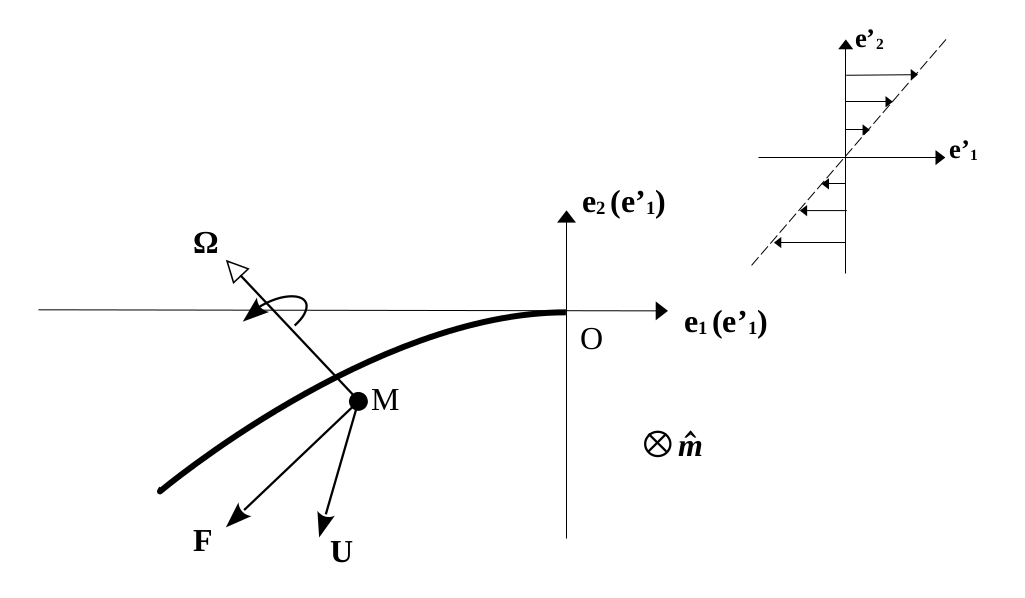
\includegraphics[width=1\textwidth]{plot/relection_general.png}
		\caption{Schematic of an elastic particle of arbitrary shape immersed in shear flow.}
    \label{fig:4}
	\end{center}
	%	\setlength{\abovecaptionskip}{-0.5 cm}
\end{figure}

Through the above analysis, we have transformed the three-dimensional problem into a two-dimensional one. We stipulate that the placement of the frames $\{\mathbf{e'_1},\mathbf{e'_2},\mathbf{e'_3}\}$ and $\{\mathbf{e_1},\mathbf{e_2},\mathbf{e_3}\}$ must satisfy $\mathbf{e'_3}=\mathbf{e_3}$. It enables us to characterize the positional relationship between the two frames using only a single variable, the orientation $\theta(t)$, as shown in Figure \ref{fig:3} (centre and right), which completely describes the relationship between the two frames.




\chapter{Theoretical Framework}
In this chapter, we present all the theoretical aspects underlying this project, including sections on mathematical modelling and its implementation.

\section{Fluid-solid interaction}
In the previous chapter, we have reduced the dimensions of the problem from three to two. Generally speaking, we will investigate a two-dimensional problem concerning the deformation and motion of a slender elastic particle in shear flow at a low Reynolds number, focussing on the particle's orientation and trajectory when it reaches equilibrium in the fluid. As this project concerns both fluid and solid mechanics, we will introduce these two components separately and then integrate them to discuss the fluid-solid interaction.
\subsection{Fluid mechanics}
We set the undeformed slender elastic particle clamped at the origin of the laboratory reference frame $\{\mathbf{e'_1}, \mathbf{e'_2}, \mathbf{e'_3}\}$ as
$\mathbf{r}_0^*(\xi^*)=(0,\xi^*)^T$, where $\xi^*\in [0,\mathcal{L}]$. We then assume that its deformed state is given by $\mathbf{R}_0^*(t^*,\xi^*)$. 
Final position of the deformed particle after translation and rotation is determined as follows:
\begin{equation}
	\label{eqn:19}
\mathbf{R}^*(t^*,\xi^*)=\bm{\mathcal{R}}\,\mathbf{R}_0^*(t^*,\xi^*)+\mathbf{r}_b^*(t^*),
\end{equation}
where $\bm{\mathcal{R}}=\left(\begin{aligned}
		&\cos(\phi(t))\quad -\sin(\phi(t)) \\
		&\sin(\phi(t))\quad \cos(\phi(t))
	\end{aligned}\right)$ is the rotation matrix with $\phi(t)$ which measures the particle's inclination as shown in Figure \ref{fig:5}, and $\textbf{r}_b^*(t^*)$ represents the translation of the particle. Note that inclination $\phi(t)$ refers to the actual rotational angle of the object. From Figure \ref{fig:5}, we can easily derive the relationship between orientation and inclination as follows:
\begin{equation}
	\label{eqn:20}
\theta(t)=\frac{\pi}{2}-\phi(t).
\end{equation}
\begin{figure}[htb]
	\begin{center}
		% specify width as 80% of the width of the text on the page
		% we can also specify a width in centimetres, e.g. [width=8cm]
		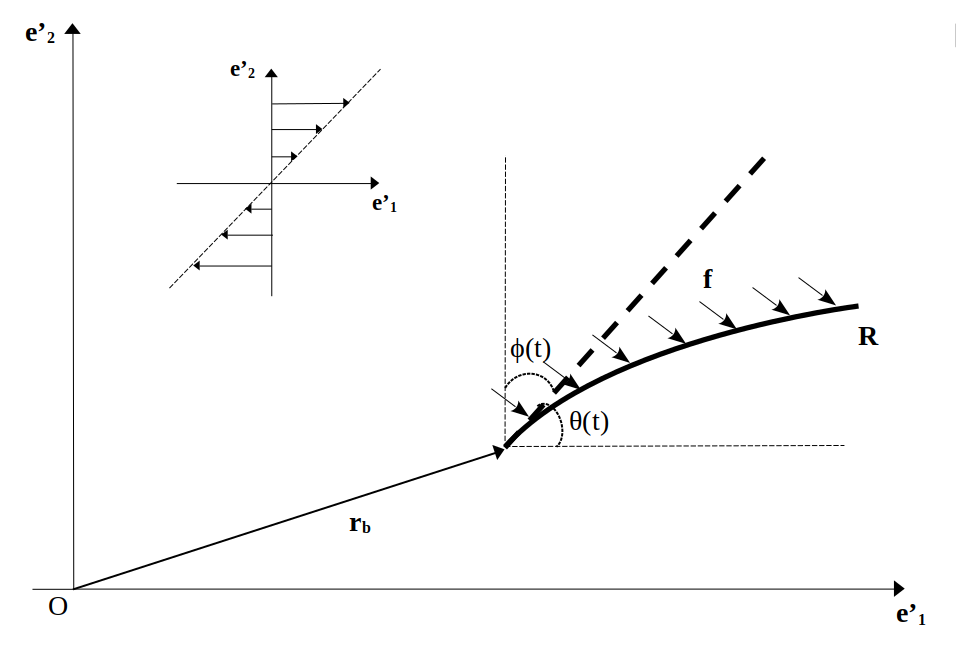
\includegraphics[width=1\textwidth]{plot/fluid_general.png}
		\caption{Schematic of a slender elastic particle in the deformed state in shear flow. The dashed black line represents its undeformed configuration.}
    \label{fig:5}
	\end{center}
	%	\setlength{\abovecaptionskip}{-0.5 cm}
\end{figure}
Since we consider a slender elastic particle immersed in shear flow, the velocity of the background flow, from \eqref{eqn:104}, is given by
\begin{equation}
\label{eqn:21}
	\mathbf{U}^{\infty*}(\mathbf{R}^*(t^*,\xi^*))=\dot{\gamma}\left(\mathbf{R}^*(t^*,\xi^*)\cdot\mathbf{e}_y\right)\cdot\mathbf{e}_x,
\end{equation}
where $\mathbf{e}_x=(1,0)^T$ and $\mathbf{e}_y=(0,1)^T$ are both unit vectors. Then, the particle's velocity from kinematics is 
\begin{equation}
\label{eqn:22}
	\mathbf{U}^*=\frac{\partial\mathbf{R}^*(t^*,\xi^*)}{\partial t^*}.
\end{equation}
Let us define a tangential vector to surface of the particle:
\begin{equation}
\label{eqn:23}
	\mathbf{e}_t=\frac{1}{|\frac{\partial\mathbf{R}^*(t^*,\xi^*)}{\partial\xi^*}|}\frac{\partial\mathbf{R}^*(t^*,\xi^*)}{\partial\xi^*}.
\end{equation}
From the slender body theory, the traction is obtained as flows:
\begin{equation}
	\label{eqn:24}
	\mathbf{f}^*=c_\perp\left(\mathbf{I}-\frac{1}{2}\mathbf{e}_t\mathbf{e}_t\right)\cdot(\mathbf{U}^{\infty*}-\mathbf{U}^*),
\end{equation}
where $c_\perp=\frac{4\pi\mu}{\ln{\frac{1}{\epsilon}}}$ is the drag coefficient \cite{KIM199147}. 

We non-dimensionalise the variables mentioned in this section using the following basic relationships:
\begin{equation}
	\label{eqn:25}
	\xi^*=\mathcal{L}\xi, \quad t^*=\frac{1}{\dot{\gamma}}\,t,
\end{equation}
where the non-dimensional variables are identified without asterisks.
Hence, the relationship between dimensional and non-dimensional variables are given by
\begin{equation}
	\label{eqn:26}
	(\mathbf{r}_0^*, \mathbf{r}_b^*, \mathbf{R}_0^*, \mathbf{R}^*)^T=\mathcal{L}\cdot(\mathbf{r}_0, \mathbf{r}_b, \mathbf{R}_0, \mathbf{R})^T,
\end{equation}
\begin{equation}
	\label{eqn:27}
\mathbf{U}^{\infty*}=\mathcal{L}\dot{\gamma}\mathbf{U}^{\infty}, \quad \mathbf{U}^*=\mathcal{L}\dot{\gamma}\mathbf{U},
\end{equation}
\begin{equation}
	\label{eqn:28}
\mathbf{f}^*=c_\perp\,\mathcal{L}\,\dot{\gamma}\,\left(\mathbf{I}-\frac{1}{2}\mathbf{e}_t\mathbf{e}_t\right)\cdot(\mathbf{U}^{\infty}-\mathbf{U})=c_\perp\,\mathcal{L}\,\dot{\gamma}\,\mathbf{f}_{f},
\end{equation}
where 
\begin{equation}
	\label{eqn:101}
\mathbf{f}_f=\left(\mathbf{I}-\frac{1}{2}\mathbf{e}_t\mathbf{e}_t\right)\cdot(\mathbf{U}^{\infty}-\mathbf{U}),
\end{equation}
is the non-dimensional fluid traction.

\subsection{Solid mechanics}
We are considering the fluid-solid interaction, so next we will focus on the part related to solid mechanics. This report employs geometrically nonlinear Kirchhoff-Love beam theory with incrementally linear constitutive equations to describe the deformation issues of elastic beams subjected to forces in fluid. We define the deformation of the beam as the dimensionless centreline displacement, $\bm{\omega} = \frac{\bm{\omega}^*}{\mathcal{L}}$. The position of a material point on the beam's centerline is denoted by 
\begin{equation}
	\label{eqn:61}
\mathbf{r}_0(\xi^1, \xi^2=0)=\mathbf{r}^0_0(\xi^1),\quad \xi^1\in [0,1].
\end{equation}
Then the position of an arbitrary point in the undeformed beam is given by 
\begin{equation}
	\label{eqn:62}
\mathbf{r}_0(\xi^1, \xi^2)=\mathbf{r}^0_0(\xi^1)+\xi^2\mathbf{n},\quad \xi^2\in [-\frac{h}{2},\frac{h}{2}],
\end{equation}
where $\mathbf{n}=(1,0)^T$ is the normal vector to the undeformed centerline, and $\frac{h}{2}=\frac{h^*}{2\mathcal{L}}$ is the non-dimensional radius of the cross section of the beam. After the deformation, the previous position $\mathbf{r}^0_0(\xi^1)$ in the undeformed reference configuration is transformed to a new position 
\begin{equation}
	\label{eqn:63}
\mathbf{R}^0_0(\xi^1)=\mathbf{r}^0_0(\xi^1)+\bm{\omega}(\xi^1).
\end{equation}
We decompose the displacement $\bm{\omega}$ into the undeformed basis:
\begin{equation}
	\label{eqn:64}
\bm{\omega}=\omega^1\mathbf{a}_1+\omega^2\mathbf{a}_2,
\end{equation}
where $\mathbf{a}_1=\frac{\partial \mathbf{r}^0_0}{\partial\xi^1}$ and $\mathbf{a}_3=\mathbf{n}$. The Kirchhoff-Love assumption states that material lines, which were normal to the undeformed centreline, remain normal to the deformed centreline and remain unstretched. Therefore, an arbitrary material point $\mathbf{r}_0$ after deformation is given by 
\begin{equation}
	\label{eqn:65}
\mathbf{R}_0(\xi^1,\xi^2)=\mathbf{R}^0_0(\xi^1)+\xi^2\mathbf{N},
\end{equation}
where $\mathbf{N}$ is the normal to the deformed configuration.

We then give the non-dimensional equation by scaling the stresses and the applied traction on the beam's effective Young's modulus
\begin{equation}
	\label{eqn:29}
E_{eff}=\frac{E}{(1-v^2)},
\end{equation}
where $E$ is the Young's modulus and $v$ is the Poisson ratio. Thus, the dimensional and non-dimensional variables are related by 
\begin{equation}
	\label{eqn:30}
		\left(\begin{aligned}
		&\mathbf{f^*} \\
		&\mathbf{\sigma}_0^*
	\end{aligned}\right)
 =E_{eff}\left(\begin{aligned}
	&\textbf{f}_{s} \\
	&\mathbf{\sigma}_0
\end{aligned}\right),
\end{equation}
where $\textbf{f}_{s}$ is the non-dimensional solid traction and $\sigma^*_0$ indicates the prestress of the elastic beam.
The non-dimensional form of the principle of virtual displacements that governs the beams deformation is then given by
\begin{equation}
	\label{eqn:31}
	\int^1_0 \left[(\sigma_0+\gamma)\delta\gamma+\frac{1}{12}h^2\kappa\delta\kappa-\left(\frac{1}{h}\sqrt{\frac{A}{a}}\,\textbf{f}_{s}-\Lambda^2\frac{\partial^2\textbf{R}_0}{\partial t^2}
	\right)\cdot \delta \textbf{R}_0
	\right]\,\sqrt{a}\,d\xi=0,
\end{equation}
where 
\begin{equation}
	\label{eqn:32} a=\frac{\partial\textbf{r}_0}{\partial\xi}\cdot\frac{\partial\textbf{r}_0}{\partial\xi}, A=\frac{\partial\textbf{R}_0}{\partial\xi}\cdot\frac{\partial\textbf{R}_0}{\partial\xi}
\end{equation}
 denote the squares of the lengths of infinitesimal material line elements in the undeformed and deformed configurations, respectively.
Also, considering undeformed and deformed ones, we have 
\begin{equation}
	\label{eqn:33}
ds=\sqrt{a}\,d\xi,\,dS=\sqrt{A}\,d\xi.
\end{equation}
$A$ and $a$ could be understood as the "$1\times1$ metric tensors" of the beam's centerline, representing the deformed and undeformed configurations, respectively. 
The ratio $\sqrt{\frac{A}{a}}$ signifies the "extension ratio" or "stretch" of the beam's centerline. We define the curvature of the beam's centerline prior to and following deformation as represented by 
\begin{equation}
	\label{eqn:34}
	b=\textbf{n}\cdot\frac{d^2\textbf{r}_0}{d\xi^2},\,B=\textbf{N}\cdot\frac{\partial^2\textbf{R}_0}{\partial\xi^2}.
\end{equation}
The "$1\times1$" strain and bending "tensors" $\gamma$ and $\kappa$ are obtained by
\begin{equation}
	\label{eqn:35}
\gamma=\frac{1}{2}(A-a),\,\kappa=-(B-b).
\end{equation}
In $\eqref{eqn:31}$,
\begin{equation}
	\label{eqn:36}
	\Lambda=\mathcal{L}\,\dot{\gamma}\sqrt{\frac{\rho}{E_{eff}}}
\end{equation}
represents the ratio of the natural timescale of the beam's in-plane extensional oscillations. 
$\Lambda^2$ can be treated as the non-dimensional wall density, implying that $\Lambda=0$ signifies the absence of wall inertia.

Since the elastic beam is initially clamped at the origin, the boundary conditions are
\begin{equation}
    \label{eqn:58}
	\mathbf{R}_0(\xi=0)\cdot\mathbf{e}_x=0,
\end{equation}
\begin{equation}
    \label{eqn:59}
	\mathbf{R}_0(\xi=0)\cdot\mathbf{e}_y=0,
\end{equation}
\begin{equation}
    \label{eqn:60}
	\frac{d\left(\mathbf{R}_0(\xi=0)\cdot\mathbf{e}_x\right)}{d\xi}=0.
\end{equation}

\subsection{Fluid–solid coupling}
The no-slip boundary condition requires that the velocity of the fluid on the surface of the beam $\mathbf{u}$ matches the velocity of the beam at that location. Hence, the boundary condition is 
\begin{equation}
    \label{eqn:100}
	\mathbf{u}=\frac{\partial \mathbf{R}(t,\xi)}{\partial t}.
\end{equation}

Recall that in $\eqref{eqn:28}$, we use slender body theory to evaluate the traction exerted by the fluid on the beam as
\begin{equation}
	\label{eqn:102}
\mathbf{f}^*=c_\perp\,\mathcal{L}\,\dot{\gamma}\,\mathbf{f}_{f}.
\end{equation}
From \eqref{eqn:30}, the applied traction on beam is 
\begin{equation}
	\label{eqn:103}
\mathbf{f}^*=E_{eff}\,\mathbf{f}_{s}.
\end{equation}
Hence, the fluid applies traction to the beam, and the loading term in the solid equation \eqref{eqn:31} are expressed by
\begin{equation}
    \label{eqn:37}
	\textbf{f}_{s}=\frac{c_\perp\,\mathcal{L}\,\dot{\gamma}}{E_{eff}}\,\textbf{f}_{f}.
\end{equation}
Then, we define the coefficient in \eqref{eqn:37} as $\mathcal{I}$, which represents the coefficient of fluid-solid interaction and is expressed as:
\begin{equation}
	\label{eqn:38}
	\mathcal{I}=\frac{c_\perp\,\mathcal{L}\,\dot{\gamma}}{E_{eff}}.
\end{equation}
This coefficient, also known as the FSI coefficient, quantifies the degree or strength of the interaction between the fluid and the solid within the system.




\section{Equilibrium equations and implementation}
We are particularly interested in the equilibrium solutions of an elastic particle in shear flow, rather than the trivial tumbling state. In this section, we establish the equilibrium equations for the problem and apply the finite element method with the Newton method to solve the system. Before this, we will first explore solutions with constant orientations, which will also assist in determining the non-dimensional expression for the translational term $\mathbf{r}_b$.

\subsection{Solutions with constant orientations}
It is worth studying further the solutions of the system with constant orientations (Namely, from \eqref{eqn:20}, we seek the steady solution for inclination $\phi(t)$, $\dot{\phi}(t)=0$), hence the following conditions  are made:
\begin{equation}
	\label{eqn:39}
	\phi(t)=\phi_{eq},\, \textbf{R}_0(t,\xi)=\textbf{R}_0(\xi).
\end{equation}
Thus, from \eqref{eqn:19} we obtain the following expressions in non-dimensional form with the conditions above:
\begin{equation}
	\label{eqn:40}
	\textbf{R}(t,\xi)=\bm{\mathcal{R}}\,\textbf{R}_0(\xi)+\textbf{r}_b(t),
\end{equation}
where $\bm{\mathcal{R}}=\left(\begin{aligned}
	&\cos(\phi_{eq})\quad -\sin((\phi_{eq}) \\
	&\sin((\phi_{eq})\quad \cos((\phi_{eq})
\end{aligned}\right) $ is the rotation matrix with $\phi(t)=\phi_{eq}$. We define $\textbf{r}_b(t)=\left(\begin{aligned}
&r_b^{1}(t) \\
&r_b^{2}(t)
\end{aligned}\right)$, and derive the following few non-dimensional formulas:
\begin{equation}
	\label{eqn:41}
	\textbf{U}^{\infty}=\left(\textbf{R}(t,\xi)\cdot\textbf{e}_y\right)\cdot\textbf{e}_x=\left((\bm{\mathcal{R}}\,\textbf{R}_0(\xi)+\textbf{r}_b(t))\cdot\textbf{e}_y\right)\cdot\textbf{e}_x.
\end{equation}
\begin{equation}
	\label{eqn:42}
	\textbf{U}=\frac{\partial\textbf{R}(t,\xi)}{\partial t}=\dot{\textbf{r}}_b(t)=\left(\begin{aligned}
		&\dot{r}_b^{1}(t) \\
		&\dot{r}_b^{2}(t)
	\end{aligned}\right).
\end{equation}
\begin{equation}
	\label{eqn:43}
	\textbf{e}_t(\xi)=\frac{1}{|\frac{\partial\textbf{R}(t,\xi)}{\partial\xi}|}\frac{\partial\textbf{R}(t,\xi)}{\partial\xi}.
\end{equation}
\begin{equation}
	\label{eqn:44}
	\textbf{f}_{f}=\left(\mathbf{I}-\frac{1}{2}\textbf{e}_t\textbf{e}_t\right)\cdot(\textbf{U}^{\infty}-\textbf{U}).
\end{equation}
From $\eqref{eqn:44}$, it can be observed that the term $\left(\mathbf{I}-\frac{1}{2}\textbf{e}_t\textbf{e}_t\right)$ is independent of time $t$. We can just analyze $(\textbf{U}^{\infty}-\textbf{U})$ to determine whether the $\textbf{f}_{f}$ is the function of time $t$ or not. Hence, we have 
\begin{equation}
	\label{eqn:45}
	\begin{aligned}
\textbf{U}^{\infty}-\textbf{U}&=\left((\bm{\mathcal{R}}\,\textbf{R}_0(\xi)+\textbf{r}_b(t))\cdot\textbf{e}_y\right)\cdot\textbf{e}_x-\dot{\textbf{r}}_b(t)\\
&=\left((\bm{\mathcal{R}}\,\textbf{R}_0(\xi))\cdot\textbf{e}_y\right)\cdot\textbf{e}_x+(\textbf{r}_b(t)\cdot\textbf{e}_y)\cdot\textbf{e}_x-\dot{\textbf{r}}_b(t)\\
&=\left((\bm{\mathcal{R}}\,\textbf{R}_0(\xi))\cdot\textbf{e}_y\right)\cdot\textbf{e}_x+\left(\begin{aligned}
	r_b^{2}&(t)\\
    0&
\end{aligned}\right)-\left(\begin{aligned}
&\dot{r}_b^{1}(t) \\
&\dot{r}_b^{2}(t)
\end{aligned}\right).
\end{aligned}
\end{equation}
From the last step of $\eqref{eqn:45}$, it is obvious that $\left((\bm{\mathcal{R}}\,\textbf{R}_0(\xi))\cdot\textbf{e}_y\right)\cdot\textbf{e}_x$ is independent of time $t$. Thus, if 
\begin{equation}
	\label{eqn:46}
\left(\begin{aligned}
	r_b^{2}&(t)\\
	0&
\end{aligned}\right)-\left(\begin{aligned}
	&\dot{r}_b^{1}(t) \\
	&\dot{r}_b^{2}(t)
\end{aligned}\right)=\textbf{0},
\end{equation}
then $(\textbf{U}^{\infty}-\textbf{U})$ is independent of time $t$, implying that $\textbf{f}_{f}$ is also independent of $t$.
Considering $\eqref{eqn:46}$, we derive the non-dimensional specific expression for $\textbf{r}_b(t)$ as follows:
\begin{equation}
	\label{eqn:47}
\textbf{r}_b(t)=\left(\begin{aligned}
		\frac{1}{2}V t^2+&U_0t+X_0\\
		Vt&+Y_0
	\end{aligned}\right),
\end{equation}
where $V$ represents the vertical drift speed and the change rate  of horizontal motion, while $U_0$ denotes the initial horizontal speed. $(X_0, Y_0)$ is the initial position of the clamped point.

In summary, due to our focus on the steady solution of the beam's inclination, we specified $\dot{\phi}(t)=0$. From the mathematical derivation above, we observe that if $\eqref{eqn:47}$ holds, the fluid traction $\textbf{f}_{f}$ is steady (independent of time $t$). This aligns with the previously established condition $\textbf{R}_0(t,\xi)=\textbf{R}_0(\xi)$. Consequently, it turns out that conditions $\eqref{eqn:39}$ are reasonable, and the entire deduction is self-consistent.

\subsection{Equilibrium equations}
Based on the conclusions drawn above, we investigate the deformation and motion of an elastic beam in the equilibrium state within shear flow. Simply put, for this system, we currently have these unknowns: $\textbf{R}_0(\xi), V, U_0$ and $\phi_{eq}$. Therefore, we need to establish the relevant equations to solve them. Note that for $\textbf{r}_b(t)$, we treat $X_0$ and $Y_0$ as constants here.

Initially, the elastic beam is clamped at the origin, denoted by $\textbf{r}_0(\xi)=(0,\xi)^T,\,\xi\in [0,1]$. Next, a traction $\mathbf{f}_s=\mathcal{I}\,\textbf{f}_0$  is applied to it, causing deformation denoted as $\textbf{R}_0(\xi)$. Substituting 
$\textbf{r}_0(\xi), \textbf{f}_s$ and $\textbf{R}_0(\xi)$ into the beam's governing equation $\eqref{eqn:31}$, we obtain the following equation:
\begin{equation}
	\label{eqn:48}
	\bm{\mathcal{S}}\left(\textbf{R}_0(\xi);\textbf{f}_0,\textbf{r}_0(\xi)\right)=0,
\end{equation}
where $\textbf{R}_0(\xi)$ is the unknown and $\bm{\mathcal{S}}(\cdot)$ indicates the left hand side of $\eqref{eqn:31}$.
Subsequently, according to $\eqref{eqn:40}$, a translation and rotation are applied to 
$\textbf{R}_0(\xi)$, yielding $\textbf{R}(t,\xi)$ as:
\begin{equation}
	\label{eqn:49}
	\textbf{R}(t,\xi)=\bm{\mathcal{R}}\,\textbf{R}_0(\xi)+\textbf{r}_b(t),
\end{equation}
where $\bm{\mathcal{R}}=\left(\begin{aligned}
	&\cos(\phi_{eq})\quad -\sin((\phi_{eq}) \\
	&\sin((\phi_{eq})\quad \cos((\phi_{eq})
\end{aligned}\right) $ and $\textbf{r}_b(t)=\left(\begin{aligned}
\frac{1}{2}\,V\,t^2+&U_0\,t+X_0\\
V\,t&+Y_0
\end{aligned}\right)$. We compute the fluid traction $\textbf{f}_f$ acting on the beam $\textbf{R}(t,\xi)$ based on $\eqref{eqn:41},\eqref{eqn:42},\eqref{eqn:43}$ and $\eqref{eqn:44}$. Then, we rotate this fluid traction $\textbf{f}_f$ back by angle $\phi_{eq}$ while keeping its magnitude unchanged, obtaining traction $\textbf{f}_0$. Hence, the relationship between $\textbf{f}_0$ and $\textbf{f}_f$ is 
\begin{equation}
	\label{eqn:50}
	\textbf{f}_0=\bm{\mathcal{R}}^{-1}\,\textbf{f}_f,
\end{equation}
where $\bm{\mathcal{R}}^{-1}$ is the inverse of the rotation matrix. Then, the solid traction, which serves as the loading term in the beam equation, is represented as 
\begin{equation}
	\label{eqn:67}
	\textbf{f}_s=\mathcal{I}\,\textbf{f}_0=\mathcal{I}\,\left(\bm{\mathcal{R}}^{-1}\,\textbf{f}_f\right).
\end{equation}
From $\eqref{eqn:44}$ and $\eqref{eqn:45}$, we know that the traction $\textbf{f}_f$ is the function of $\textbf{R}_0(\xi), V, U_0$ and $\phi_{eq}$. Thus, traction $\textbf{f}_0$ is also the function of  $\textbf{R}_0(\xi), V, U_0$ and $\phi_{eq}$, that is, $\textbf{f}_0\left(\textbf{R}_0(\xi), V, U_0,\phi_{eq}\right)$. It means that $\eqref{eqn:48}$ can be updated by
\begin{equation}
	\label{eqn:51}
	\bm{\mathcal{S}}\left(\textbf{R}_0(\xi), V, U_0,\phi_{eq};\textbf{r}_0(\xi)\right)=0,
\end{equation}
where $\textbf{r}_0(\xi)=(0,\xi)^T,\,\xi\in [0,1]$ is not the unknown in this equation.

The net drag and net torque acting on the beam $\textbf{R}(t,\xi)$ in non-dimensional form are 
\begin{equation}
\label{eqn:52}
\textbf{F}=\int^1_0 \textbf{f}\, \left|\frac{\partial\textbf{R}}{\partial\xi}\right|\,d\xi, 
\end{equation}
\begin{equation}
	\label{eqn:53}
\mathbf{T}\cdot\textbf{e}_z=\left\{\int^1_0 \left[(\textbf{R}-\textbf{R}_{centre})\times \textbf{f}\,\right]\,\left|\frac{\partial\textbf{R}}{\partial\xi}\right|\,d\xi\right\}\cdot\textbf{e}_z,
\end{equation}
where 
\begin{equation}
	\label{eqn:54}
\textbf{R}_{centre}=\int^1_0 \textbf{R}\,|\frac{\partial\textbf{R}}{\partial\xi}|\,d\xi
\end{equation}
represents the position of centre of mass. Since we are investigating the equilibrium state of the elastic beam in shear flow, the net drag and net torque experienced by the beam are both zero. Hence, we have 
\begin{equation}
	\label{eqn:55}
\textbf{F}\,(\textbf{R}_0(\xi), V, U_0, \phi_{eq})=\textbf{0},
\end{equation}
\begin{equation}
	\label{eqn:56}
	\{\mathbf{T}\cdot\textbf{e}_z\}\,(\textbf{R}_0(\xi), V, U_0, \phi_{eq})=0.
\end{equation} 
Combining $\eqref{eqn:51}, \eqref{eqn:55}$ and $\eqref{eqn:56}$, we collect the following equations for unkonwns:
\begin{equation}
	\label{eqn:57}
	\left\{\begin{aligned}
&\bm{\mathcal{S}}\left(\textbf{R}_0(\xi), V, U_0,\phi_{eq};\textbf{r}_0(\xi)\right)=0\\
&\textbf{F}\,(\textbf{R}_0(\xi), V, U_0, \phi_{eq})=\textbf{0}\\
&\{\mathbf{T}\cdot\textbf{e}_z\}\,(\textbf{R}_0(\xi), V, U_0, \phi_{eq})=0
\end{aligned}\right.\Longrightarrow \left(\textbf{R}_0(\xi), V, U_0, \phi_{eq}\right).
\end{equation}
By solving the system of equations $\eqref{eqn:57}$, we can obtain the parameters necessary to describe the deformation and motion of the elastic beam in shear flow when it is in equilibrium. 

\subsection{Implementation}
We use the finite element method in conjunction with Newton method to solve the governing equations \eqref{eqn:57} numerically. Given that the beam's governing equation is expressed in the form of variation with virtual displacement $\delta \mathbf{R}_0$, we shall first discretise it.


We restate the beam's governing equation $\eqref{eqn:31}$ here:
\begin{equation}
	\label{eqn:66}
	\int^1_0 \left[(\sigma_0+\gamma)\delta\gamma+\frac{1}{12}h^2\kappa\delta\kappa-\left(\frac{1}{h}\sqrt{\frac{A}{a}}\,\textbf{f}_{s}-\Lambda^2\frac{\partial^2\textbf{R}_0}{\partial t^2}
	\right)\cdot \delta \textbf{R}_0
	\right]\,\sqrt{a}\,d\xi=0.
\end{equation}
In finite element method, we represent the Lagrangian coordinates as a discrete sum using known basis functions, $P_j$:
\begin{equation}
	\label{eqn:68}
	\xi=\sum_j \hat{\xi}_j\, P_j,
\end{equation}
where $\hat{\xi}_j$ is the Lagrangian coordinate at $j$-th node. Then, we take an isoparametric approach and use the same basis functions for the unknown deformed position
\begin{equation}
	\label{eqn:69}
	R^i=\sum_j \hat{R}_j^i\, P_j,\quad i=1,2,
\end{equation}
where $R^i$ is the $i$-th component of $\mathbf{R}_0$, namely $\mathbf{R}_0=(R^1, R^2)$.
Since variations in the position are determined by variations only in the discrete variables, we have 
\begin{equation}
	\label{eqn:70}
	\delta\mathbf{R}_0=\sum_j \delta\hat{R}_j^i\, P_j\mathbf{e}_i,
\end{equation}
\begin{equation}
	\label{eqn:71}
	\delta\frac{\partial\mathbf{R}_0}{\partial\xi}=\sum_j \delta\hat{R}_j^i\, \frac{\partial P_j}{\partial\xi}\mathbf{e}_i, \quad \delta\frac{\partial^2\mathbf{R}_0}{\partial\xi^2}=\sum_j \delta\hat{R}_j^i\, \frac{\partial^2 P_j}{\partial\xi^2}\mathbf{e}_i.
\end{equation}
Since the principle of virtual displacements is simply the virtual work expressed only through displacement variations, we should have
\begin{equation}
	\label{eqn:72}
	\delta\gamma=\delta\left(\frac{1}{2}(A-a)\right)=\frac{\partial\mathbf{R}_0}{\partial\xi}\cdot\delta\frac{\partial\mathbf{R}_0}{\partial\xi}=\frac{\partial\mathbf{R}_0}{\partial\xi}\cdot\sum_j \delta\hat{R}_j^i\, \frac{\partial P_j}{\partial\xi}\mathbf{e}_i,
\end{equation}
\begin{equation}
	\label{eqn:73}
	\delta\kappa=\delta\left(-(B-b)\right)=-\mathbf{N}\cdot\delta\frac{\partial^2\mathbf{R}_0}{\partial\xi^2}=-\mathbf{N}\cdot\frac{\partial^2\,\delta\mathbf{R}_0}{\partial\xi^2}=-\mathbf{N}\cdot\sum_j \delta\hat{R}_j^i\,\frac{\partial^2 P_j}{\partial\xi^2}\mathbf{e}_i.
\end{equation}
Substituting \eqref{eqn:70}, \eqref{eqn:72} and \eqref{eqn:73} into the beam's governing equation \eqref{eqn:66}, we obtain 
\begin{equation}
	\label{eqn:74}
    \begin{aligned}
	\sum_j\int^1_0 \Bigg[(\sigma_0+\gamma)\left(\frac{\partial R^i}{\partial\xi}\frac{\partial P_j}{\partial\xi}\right)&-\frac{1}{12}h^2\kappa N^i \frac{\partial^2 P_j}{\partial\xi^2}\\
 &-\left(\frac{1}{h}\sqrt{\frac{A}{a}}\,f^i_{s}-\Lambda^2\frac{\partial^2 R^i}{\partial t^2}
	\right)P_j
	\Bigg]\delta\hat{R}_j^i\,\sqrt{a}\,d\xi=0.
    \end{aligned}
\end{equation}
The discrete variations can be moved outside the integrals because they are not functions of space
\begin{align}
    \label{eqn:75}
    \sum_j \Bigg\{ \int_0^1 \Bigg[(\sigma_0+\gamma) \left( \frac{\partial R^i}{\partial \xi} \frac{\partial P_j}{\partial \xi} \right) 
    &- \frac{1}{12} h^2 \kappa N^i \frac{\partial^2 P_j}{\partial \xi^2} \notag \\
    &- \left( \frac{1}{h} \sqrt{\frac{A}{a}} f^i_{s} - \Lambda^2 \frac{\partial^2 R^i}{\partial t^2} \right) P_j
    \Bigg] \sqrt{a} \, d\xi \Bigg\} \delta \hat{R}_j^i = 0.
\end{align}
Since the variations of the unknowns are independent, \eqref{eqn:75} can only be satisfied for all possible variations if each term in the braces is zero, resulting in one discrete equation for each unknown
\begin{equation}
	\label{eqn:76}
	\int^1_0 \left[(\sigma_0+\gamma)\left(\frac{\partial R^i}{\partial\xi}\frac{\partial P_j}{\partial\xi}\right)-\frac{1}{12}h^2\kappa N^i \frac{\partial^2 P_j}{\partial\xi^2}-\left(\frac{1}{h}\sqrt{\frac{A}{a}}\,f^i_{s}-\Lambda^2\frac{\partial^2 R^i}{\partial t^2}
	\right)P_j
	\right]\sqrt{a}\,d\xi=0.
\end{equation}

Since this is a beam problem, we use the one-dimensional, isoparametric, two-node Hermite solid mechanics elements. The Hermite shape functions are 
\begin{equation}
	\label{eqn:77}
 \begin{aligned}
         \psi_{11}(s)=\frac{1}{4}(s^3-3s+2), \quad \psi_{12}(s)=\frac{1}{4}(s^3-s^2-s+1),\\
         \psi_{21}(s)=\frac{1}{4}(2+3s-s^3), \quad \psi_{22}(s)=\frac{1}{4}(s^3+s^2-s-1),
 \end{aligned}
\end{equation}
where $s\in [-1,1]$ denotes the one-dimensional local coordinate of the element.
We decide the number of nodal points, $N$, and distribute them evenly through the domain. At each node, there are four degrees of freedom: 
\begin{equation}
    \label{eqn:87}
    \mathbf{R}_0\cdot\mathbf{e}_x, \quad\mathbf{R}_0\cdot\mathbf{e}_y, \quad\frac{d\left(\mathbf{R}_0\cdot\mathbf{e}_x\right)}{d\xi},\quad\frac{d\left(\mathbf{R}_0\cdot\mathbf{e}_y\right)}{d\xi}.
\end{equation}
However, based on the boundary conditions (restate here): 
\begin{equation}
    \label{eqn:85}
    \begin{aligned}
      &\mathbf{R}_0(\xi=0)\cdot\mathbf{e}_x=0, \\
      &\mathbf{R}_0(\xi=0)\cdot\mathbf{e}_y=0,\\
      &\frac{d\left(\mathbf{R}_0(\xi=0)\cdot\mathbf{e}_x\right)}{d\xi}=0,
    \end{aligned}
\end{equation}
we know that at node $1$ (when $j=1$), there is only one degree of freedom $\frac{d\left(\mathbf{R}_0(\xi=0)\cdot\mathbf{e}_y\right)}{d\xi}$, while the other three are pinned.
Now, \eqref{eqn:69} is expressed as
\begin{equation}
	\label{eqn:79}
    R^i=\sum_{j=2}^{N} \sum_{k=1}^2 \hat{R}_{ijk}\,\psi_{jk}+(i-1)\hat{R}_{212}\,\psi_{12}, \quad i=1,2,
\end{equation}
where $\hat{R}_{ij1}$ represents the $i$-th coordinate of the node $j$ and $\hat{R}_{ij2}$ represents the derivative of $i$-th coordinate with respect to $\xi$, evaluated at the node $j$. Note that $\psi_{jk}$ is a function of $\xi$. By substituting the Hermite shape functions into \eqref{eqn:68}, the interpolation expression for $\xi(s)$ is obtained as:
\begin{equation}
	\label{eqn:99}
    \xi=\sum_j\sum_k \hat{\xi}_{jk}\, \psi_{jk}(s).
\end{equation}
Thus, within each element, the local coordinate $s$ can be expressed in terms of $\xi$.
Then, we set that 
\begin{equation}
	\label{eqn:88}
    \begin{aligned}
    (X_1, ..., X_m, ...,X_{4N-3})=&(\hat{R}_{121},...,\hat{R}_{1N1},\hat{R}_{122},...,\hat{R}_{1N2},\\
    &\hat{R}_{221},...,\hat{R}_{2N1},\hat{R}_{212}, \hat{R}_{222},...,\hat{R}_{2N2}). 
     \end{aligned}
\end{equation}
We introduce three additional unknowns.
\begin{equation}
	\label{eqn:83}
    X_{4N-2}=V, \quad X_{4N-1}=U_0, \quad X_{4N}=\phi_{eq}.
\end{equation}
Substituting \eqref{eqn:79} and Hermite shape functions into \eqref{eqn:76}, then we define the left-hand side of the equation as the residuals $r_l$, where $l=1,...,4N-3$. From \eqref{eqn:55} and \eqref{eqn:56}, we introduce three additional residuals (drag-free and torque-free) as follows:
\begin{equation}
	\label{eqn:80}
    r_{4N-2}=F^1\,(\textbf{R}_0(\xi), V, U_0, \phi_{eq}),
\end{equation}
\begin{equation}
	\label{eqn:81}
    r_{4N-1}=F^2\,(\textbf{R}_0(\xi), V, U_0, \phi_{eq}),
\end{equation}
\begin{equation}
	\label{eqn:82}
    r_{4N}=\{\mathbf{T}\cdot\textbf{e}_z\}\,(\textbf{R}_0(\xi), V, U_0, \phi_{eq}).
\end{equation}

We use the multidimensional Newton method to solve this system. Firstly, we provide an initial guess for the unknowns and set them as $\{X^{[0]}_m\}^{4N}_1$. Then, determine the residuals $r^{[0]}_l$ for $l=1,...,4N$, and the entries in the Jacobian matrix
\begin{equation}
	\label{eqn:84}
    J_{lm}=\frac{\partial r_l}{\partial X_m} \quad \text{for}\quad l,m=1,...,4N.
\end{equation}
Next, solve the linear system
\begin{equation}
	\label{eqn:89}
    \sum_{m=1}^{4N} J_{lm}\,\delta X_m=-r_l^{[0]},\quad \text{where}\quad l=1,...,4N,
\end{equation}
for $\delta X_l$ ($l=1,...,4N$). After that, correct the initial guess by
\begin{equation}
	\label{eqn:90}
    X_m=X_m^{[0]}+\delta X_m,\quad \text{where}\quad m=1,...,4N.
\end{equation}
Now, we would have to continue the Newton iteration until the residuals $ r_l\,(l=1,...,4N) $ were sufficiently small.
Finally, substituting $\{X_m\}_1^{4N-3}$ into \eqref{eqn:79} yields the finite-element solutions $\mathbf{R}_0$, and the remaining three $\{X_m\}_{4N-3}^{4N}$ are the solutions $V,U_0,\phi_{eq}$.



\chapter{Results}
In this project, we select the boomerang shape as the initial configuration of the elastic particle. This choice is based on the work of Roggeveen and Stone \cite{roggeveen2022motion}, as this shape can qualitatively capture the behaviour of many more complex bodies and has yielded significant results for rigid materials, which holds substantial practical relevance. In this chapter, we present numerical results on the elastic boomerang particle through a series of illustrative images visualised from the data.

\section{Geometry of the particle}
This report draws on the definition of the boomerang's geometry as described in Roggeveen and Stone's paper \cite{roggeveen2022motion}, using two parameters, $q$ and $\alpha$, to characterise the shape of an elastic boomerang when it is not under any force. We define the length of the long arm of the boomerang as $l_1=q+0.5$, and the length of the short arm as $l_2=0.5-q$, where $q \in [0,0.5)$. The total length is $l_1+l_2=1$ (note that we set the total length of the particle as the characteristic length $\mathcal{L}$). Additionally, we define the angle between the two arms as the opening angle $\alpha$, where $\alpha \in (0,2\pi)$. Figure \ref{fig:1} shows the basic idea about these geometrical setups. 
\begin{figure}[htb]
	\begin{center}
		% specify width as 80% of the width of the text on the page
		% we can also specify a width in centimetres, e.g. [width=8cm]
		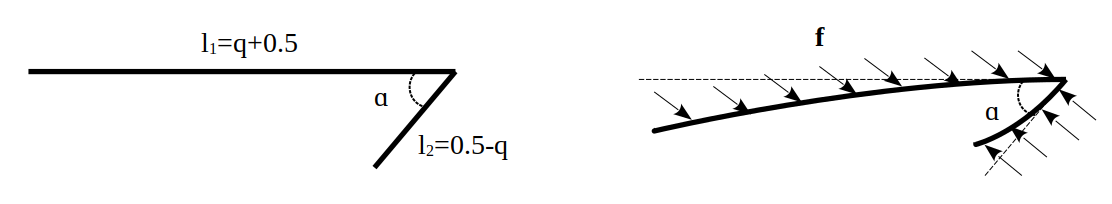
\includegraphics[width=1\textwidth]{plot/geometry.png}
		\caption{Schematics of the geometry of the boomerang. The left diagram illustrates the case without any applied force, while the right diagram shows a deformed configuration with traction $\mathbf{f}$ acting on it. As the boomerang is made of an inextensible elastic material, its total length will remain constant.}
    \label{fig:1}
	\end{center}
	%	\setlength{\abovecaptionskip}{-0.5 cm}
\end{figure}
Note that there are several extreme cases:
\begin{equation}
	\label{eqn:1}
	\left.
	\begin{aligned}
		&\alpha=0,\pi \\
		&	q=0.5
	\end{aligned}
	\right\}\Longrightarrow \text{straight rod},\quad 
	q=0, \alpha \neq 0, \pi \Longrightarrow \text{same arm length}.
\end{equation}
We exclude the case where the object becomes a straight rod (considering the ranges of $q$ and $\alpha$), as this shape yields only the trivial solution by using slender body theory. We assume that the boomerang has a small radius $\frac{h}{2}\ll \min\{l_1, l_2\}$, and define the aspect ratio $\epsilon$, which is small, such that $\epsilon=\frac{h/2}{\min\{l_1, l_2\}}\ll1$. Technically, this boomerang is an inextensible elastic composite slender object with a non-flexible hinge. 

\section{Incorporation into the algorithm}
\begin{figure}[!h]
	\begin{center}
		% specify width as 80% of the width of the text on the page
		% we can also specify a width in centimetres, e.g. [width=8cm]
		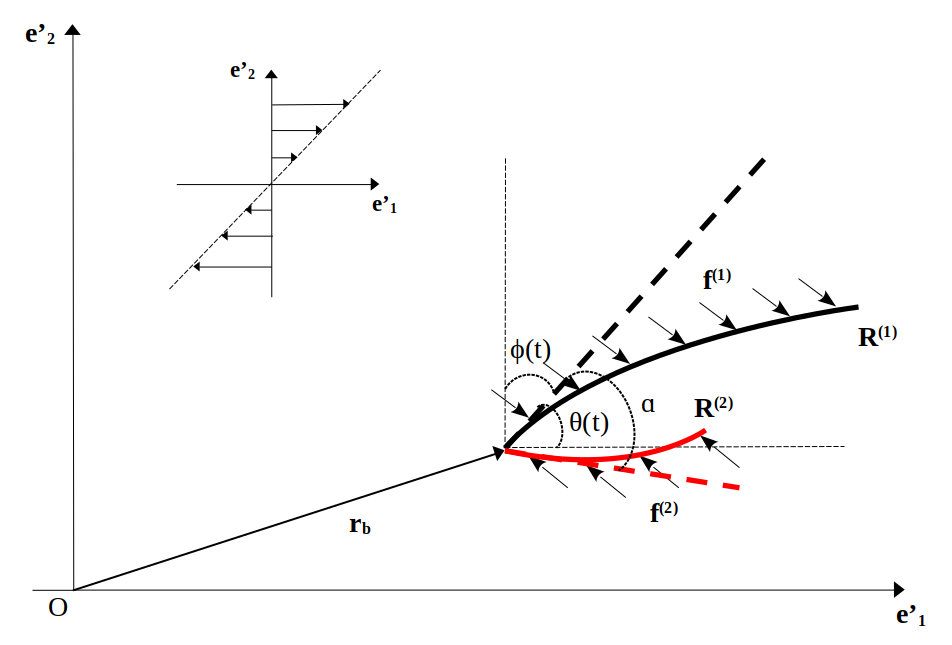
\includegraphics[width=1\textwidth]{plot/fluid.png}
		\caption{Schematic of an elastic boomerang-shaped particle in the deformed state immersed in shear flow. The dashed black and dashed red lines represent the undeformed configurations corresponding to the deformed arms $\mathbf{R}^{(1)}$ and $\mathbf{R}^{(2)}$, respectively. $\alpha$ is the opening angle between the two dashed lines.} 
    \label{fig:6}
	\end{center}
	%	\setlength{\abovecaptionskip}{-0.5 cm}
\end{figure}
To implement the algorithm for this particle, we model it as two elastic beams joined at the hinge point. Initially, both beams are clamped at the origin, differing in length and rotation angle. The length of the long beam is $q+0.5$, while the short beam's length is $0.5-q$, where $q \in [0,0.5)$. The rotation angle for the long beam is given by the inclination $\phi(t)$, whereas for the short beam, it is $\phi(t)+\alpha$. Figure \ref{fig:6} provides a schematic illustration of this process. 

Next, considering the degrees of freedom, this system is essentially a combination of two beams and three additional unknowns. From the previous analysis in Chapter 3, we know that for one beam, there are $4N-3$ degrees of freedom. Therefore, for two beams, there are $8N-6$ degrees of freedom. By adding additional unknowns $V,U_0,\phi_{eq}$, the system has a total of $8N-3$ degrees of freedom. Note that $N$ represents the number of nodal points for a single beam configuration, and we set the number of nodes to be the same for both arms of the particle.


\section{Numerical results}
Roggeveen and Stone \cite{roggeveen2022motion} have studied the dynamics of this particle shape for the rigid case, namely $\mathcal{I}=0$, in shear flow at a low Reynolds number. If, when $\mathcal{I}=0$, the solutions coincide with the results presented in their paper, it would lend a certain degree of validation to our results.
We run multiple examples using \texttt{oomph-lib} and select some representative cases to present in this report. Similar to the results of Roggeveen and Stone in Figure \ref{fig:18}, the complete solutions of the system also exhibit four solutions. Of these four fixed orientations, two differ from the other two by an angle of $\pi$ but possess the same shapes, as shown in Figure \ref{fig:20}. Hence, to simplify the discussion, we will focus solely on one group of the two solutions in the following sections.
	\begin{figure}[!h]
	\begin{center}
		% specify width as 80% of the width of the text on the page
		% we can also specify a width in centimetres, e.g. [width=8cm]
		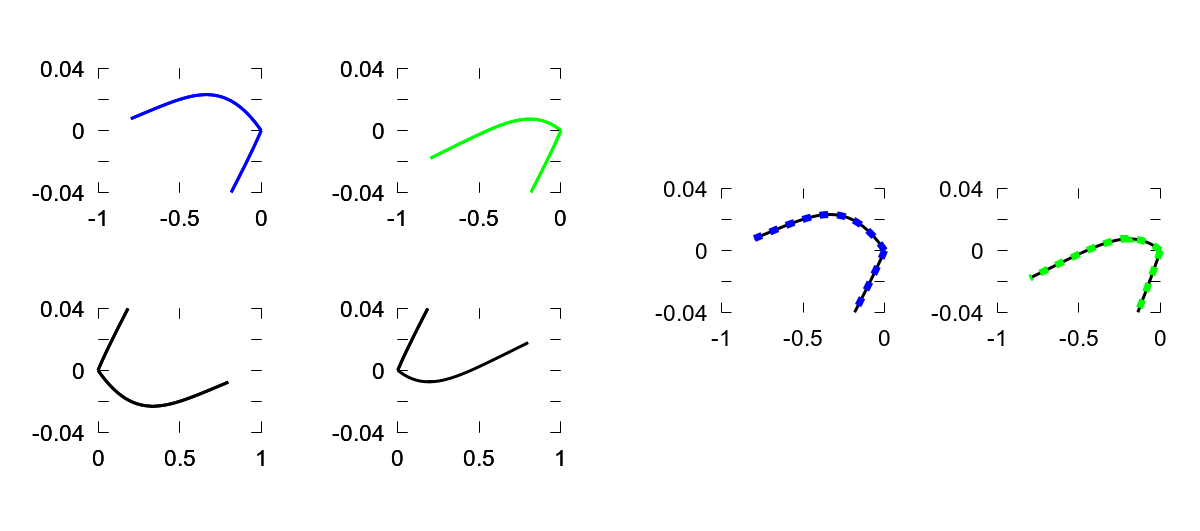
\includegraphics[width=1\textwidth]{plot/four_solutions2.png}
		\caption{Left: the complete solutions of the system for $q=0.3, \alpha=0.125\pi, \mathcal{I}=0.0003$. Right: the shapes are compared by rotating the black curve by $\pi$ to match the corresponding blue or green curve.}
    \label{fig:20}
	\end{center}
	%	\setlength{\abovecaptionskip}{-0.5 cm}
\end{figure}
	\begin{figure}[!h]
	\begin{center}
		% specify width as 80% of the width of the text on the page
		% we can also specify a width in centimetres, e.g. [width=8cm]
		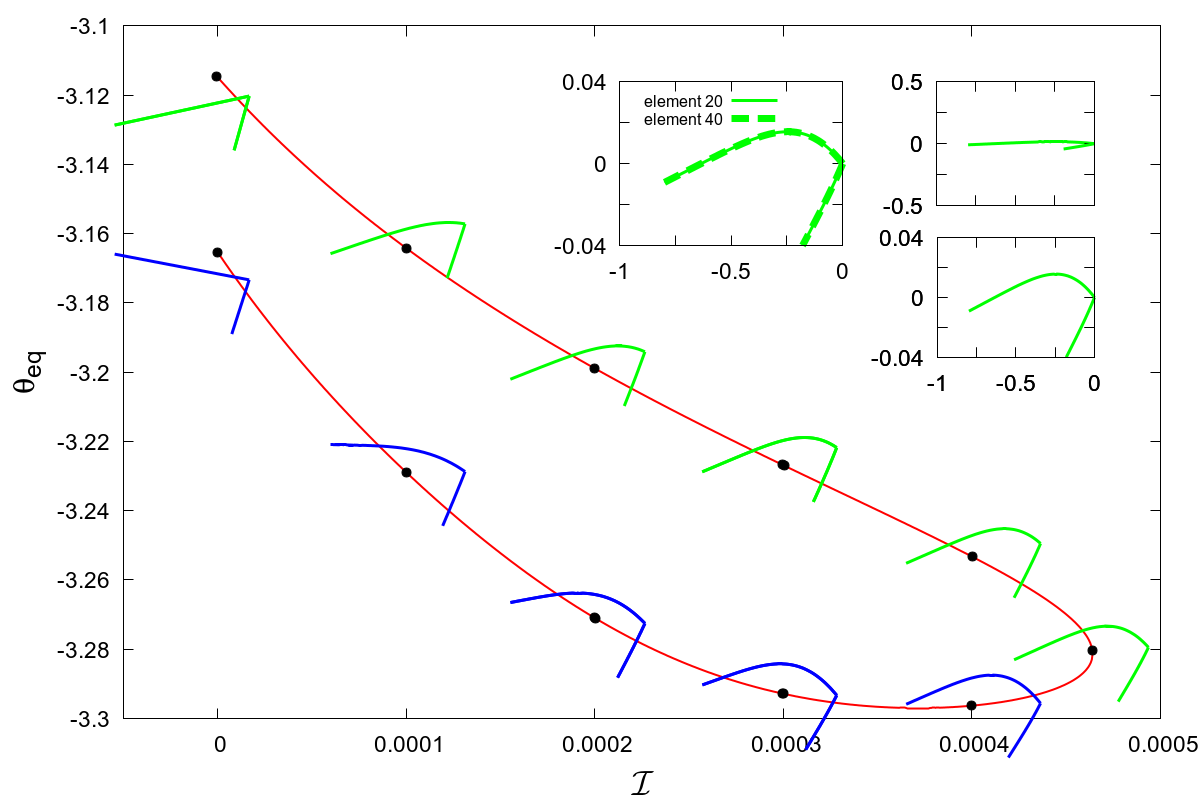
\includegraphics[width=1\textwidth]{plot/combine_elastic_beam_I_theta_q_0.30_alpha_0.125pi_initial_-4.80_0.png}
		\caption{The steady orientation $\theta_{eq}$ is plotted against the FSI coefficient $\mathcal{I}$ for the particle with shape parameters $q = 0.3$ and $\alpha = 0.125\pi$. Deformations of all shapes are amplified. In the top-right corner, a comparison between the amplified and actual shapes is provided at the limit point to illustrate the scale of deformation. We use 20 elements in solving the problem, and a convergence test, also shown in the top-right corner after doubling the number of elements, verifies that 20 elements are sufficient to accurately capture the behaviour of the system. Shapes along each branch of the curve consistently display the same colour.}
    \label{fig:7}
	\end{center}
	%	\setlength{\abovecaptionskip}{-0.5 cm}
\end{figure}

We believe that plotting the steady orientation $\theta_{eq}$ against the FSI coefficient $\mathcal{I}$ could be an effective way to initially visualise the data. Figure \ref{fig:7} illustrates the case of $q = 0.3$ and $\alpha = 0.125\pi$. The curve begins and ends at $\mathcal{I}=0$, which is consistent with the rigid case results in Roggeveen and Stone's paper \cite{roggeveen2022motion}. To intuitively demonstrate the different deformations along the curve, we also attach the shapes of the particle at various points. There is a limit point within this curve where the deformed shapes on both the upper and lower branches converge and align with each other. We observe that the long arm undergoes more noticeable deformation, while the short arm shows no significant deformation. The deformed shapes can be classified by the number of humps in the deformed long arm. In Figure \ref{fig:7}, these shapes fall into the 'one hump' category.
\begin{figure}[!h]
	\begin{minipage}[t]{1\textwidth}
		\centering
		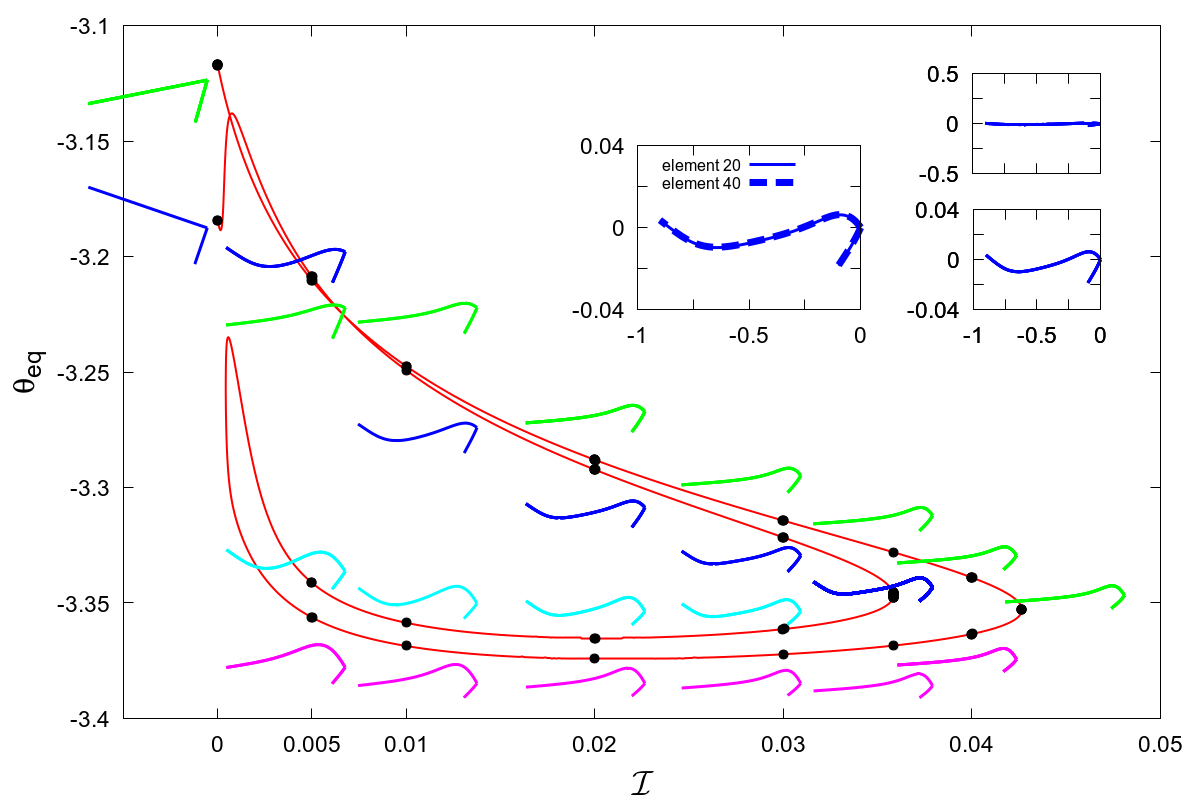
\includegraphics[width=\textwidth]{plot/combine_elastic_beam_I_theta_q_0.400_alpha_0.125pi_initial_-4.80_0.png}
	\end{minipage}
     \hfill
	\begin{minipage}[t]{1\textwidth}
		\centering
		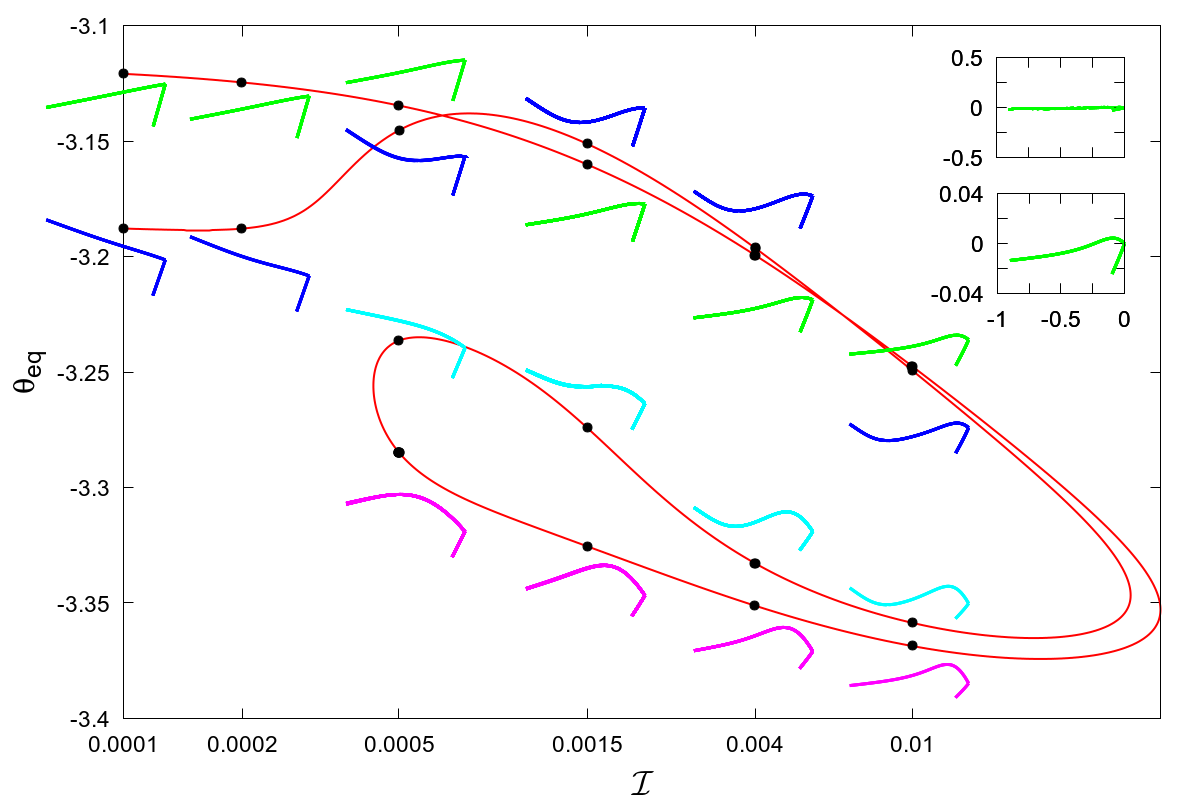
\includegraphics[width=\textwidth]{plot/initial_combine_elastic_beam_I_theta_q_0.400_alpha_0.125pi_initial_-4.80_0.png}
	\end{minipage}
	\caption{Top: the steady orientation $\theta_{eq}$ is plotted against  the FSI coefficient $\mathcal{I}$ for the particle with shape parameters $q = 0.4$ and $\alpha = 0.125\pi$. The convergence test with doubled elements is performed at one of the limit points. Bottom: the logarithmic plot for the same case, providing clearer illustration of the variations in the interval $\mathcal{I} \in [0, 0.001]$, where the curve changes significantly.}
    \label{fig:8}
\end{figure}
Figure \ref{fig:8} depicts a more complex curve than Figure \ref{fig:7}, featuring numerous twists and additional limit points. The only difference in the initial undeformed shapes between this case and that of Figure \ref{fig:7} lies in the lengths of the two arms: here, the long arm is longer and the short arm is shorter than in the previous case. This curve also begins and ends at $\mathcal{I}=0$, consistent with the rigid results from that paper \cite{roggeveen2022motion}. The shapes along the different branches ultimately align at the limit points. The outer branch of the curve is similar to Figure $\ref{fig:7}$'s case, with shapes in this branch also falling into the 'one hump' category. New shapes appear in the inner curve, where a tail develops at the end of the long arm. These shapes can be classified into the 'two humps' category. We also find that, compared to the previous case, $\mathcal{I}_{max}$ increases and $\theta_{eq,min}$ decreases. Additionally, a bifurcation occurs along the curve, revealing an even more intriguing phenomenon as $\alpha$ varies, as shown in Figure \ref{fig:9}.
\begin{figure}[!h]
	\begin{center}
		% specify width as 80% of the width of the text on the page
		% we can also specify a width in centimetres, e.g. [width=8cm]
		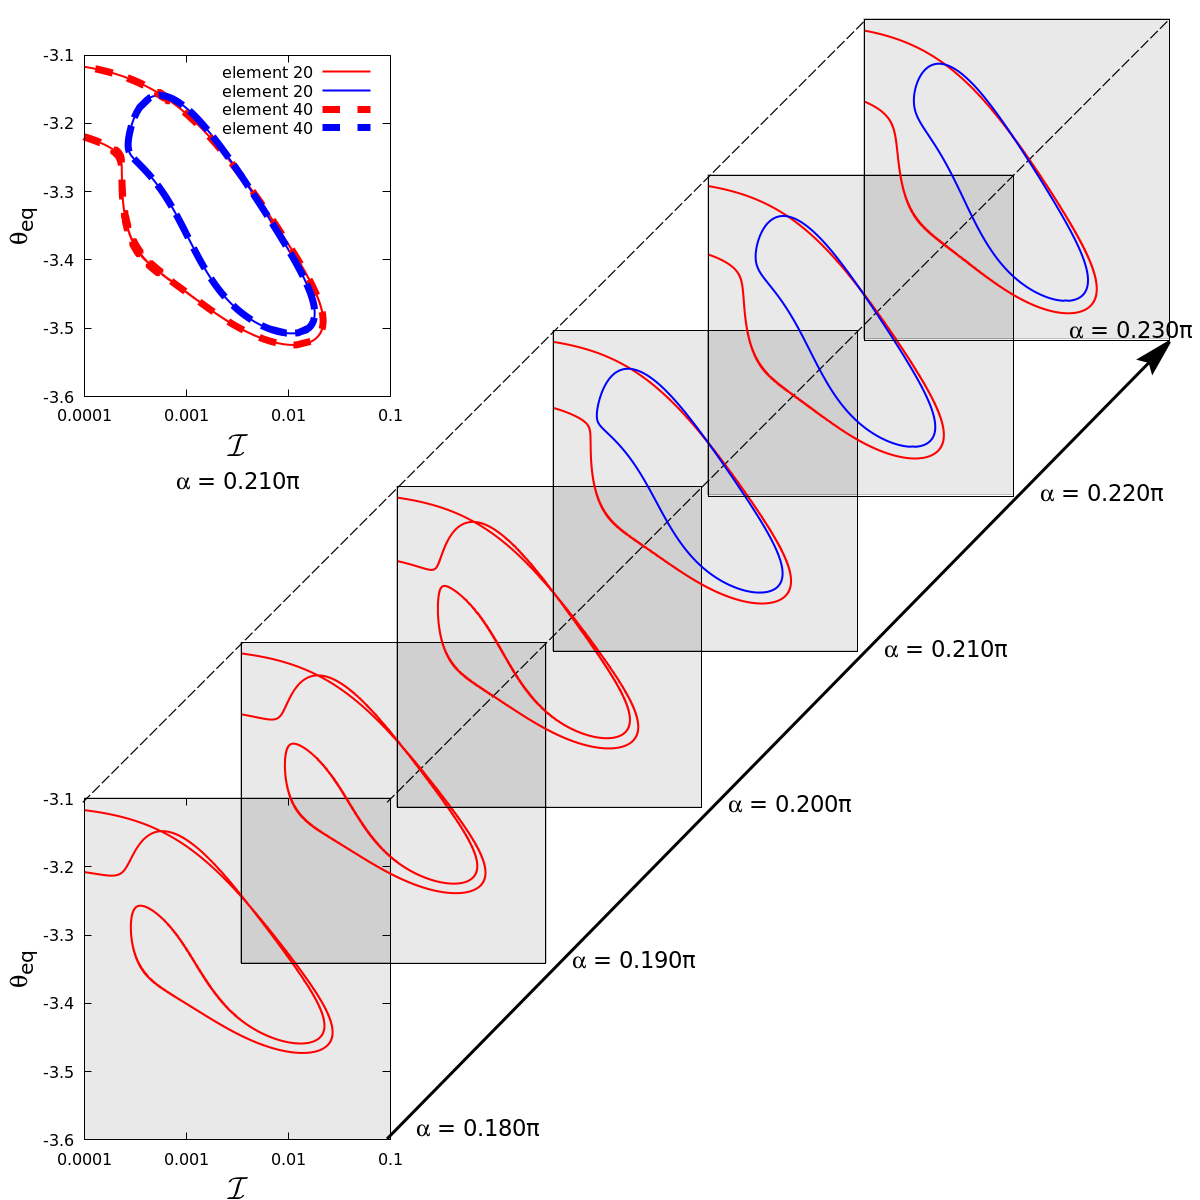
\includegraphics[width=1\textwidth]{plot/elastic_beam_I_theta_q_0.400_alpha.png}
		\caption{A sequence of logarithmic plots presents the steady orientation $\theta_{eq}$ against the FSI coefficient $\mathcal{I}$ for shape parameters $q = 0.4$ with varying $\alpha$. The top-left subplot shows the convergence test with doubled elements, and the scale of the axes is consistent across all subplots.}
   \label{fig:9}
   \end{center}
	%	\setlength{\abovecaptionskip}{-0.5 cm}
\end{figure}
Figure \ref{fig:9} is a sequence of logarithmic plots illustrating the bifurcation process as $\alpha$ increases. In the first three subplots, where $\alpha=0.180\pi,0.190\pi,0.200\pi$, the curve exhibits two prominent protrusions. As $\alpha$ increases, the distance between these protrusions gradually decreases. When $\alpha$ reaches a value between $0.200\pi$ and $0.210\pi$, a bifurcation occurs, giving rise to a new, independent inner closed loop (blue). This bifurcation signifies a critical transition in the system’s behaviour, where the previously connected equilibrium solutions split, leading to multiple distinct solution curves. We also check the shapes along the newly appeared blue curve still follow the observed pattern and belong to the 'two humps' category.

\begin{figure}[!h]
	\begin{center}
		% specify width as 80% of the width of the text on the page
		% we can also specify a width in centimetres, e.g. [width=8cm]
		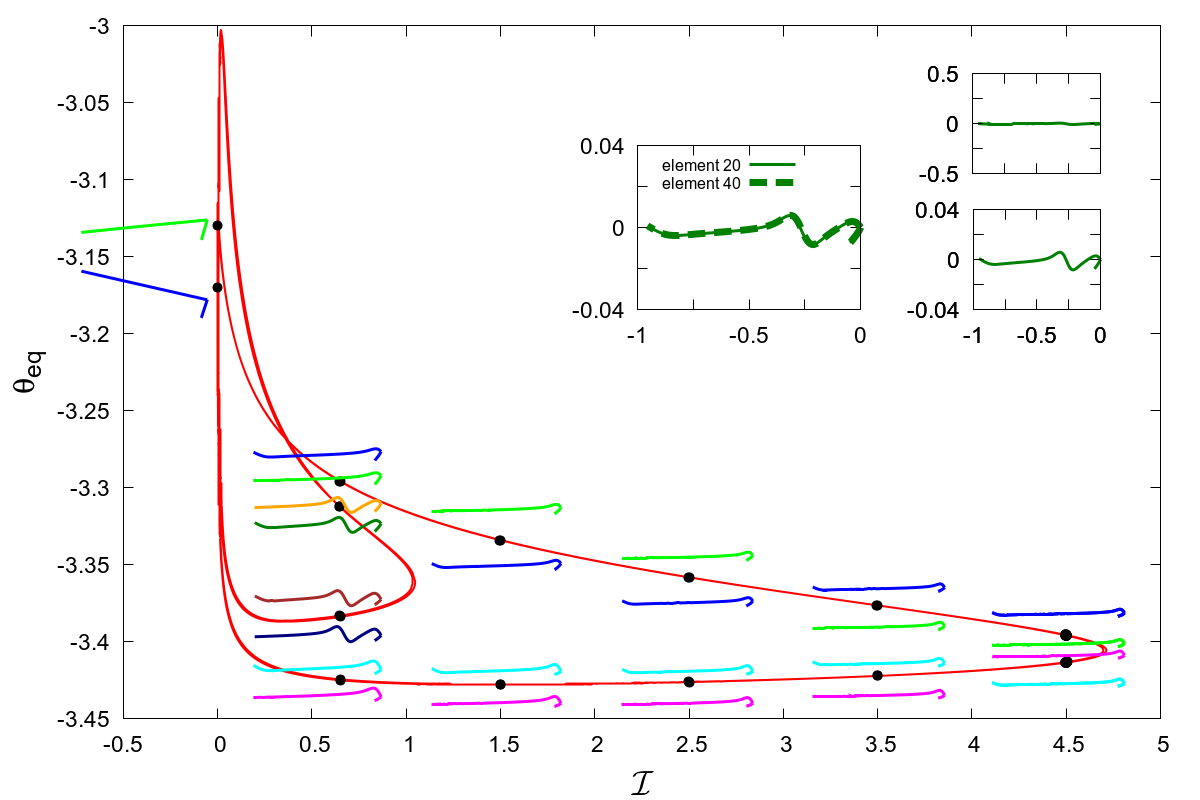
\includegraphics[width=1\textwidth]{plot/combine_elastic_beam_I_theta_q_0.452_alpha_0.125pi_initial_-4.80_0.png}
		\caption{The steady orientation $\theta_{eq}$ is plotted against the FSI coefficient $\mathcal{I}$ for the particle with shape parameters $q = 0.452$ and $\alpha = 0.125\pi$. The top-right subplot shows the convergence test with doubled elements for the case at $\mathcal{I}=0.65$.}
    \label{fig:10}
	\end{center}
	%	\setlength{\abovecaptionskip}{-0.5 cm}
\end{figure}
We find even more complex curves, and Figure \ref{fig:10} illustrates a representative case for a larger $q$, where the length of the short arm is very small. Although this curve appears complex, it still starts and ends at $\mathcal{I}=0$, maintaining consistency with the Roggeveen and Stone's results \cite{roggeveen2022motion}. The curve exhibits more twists and includes additional shape types. Intuitively, there are two new categories with corresponding new branches. In the outer new branch, the shapes (orange and dark blue) display 'three humps'. In the inner new branch, the shapes (dark green and brown) exhibit 'four humps,' with a tail forming at the end of the long arm, following the previous pattern where a tail appears in the shape on the inner branch of the curve. The two outermost branches, which are very close to each other, exhibit multiple intersections. This is why the order of the shapes (green and blue, cyan and purple) changes along these branches. The shapes along these two outermost branches still belong to the 'two humps' and 'one hump' categories. Actually, this complex curve has more bifurcations, as shown in Figure \ref{fig:11}.
\begin{figure}[!h]
	\centering
	\begin{minipage}{\linewidth}
		\centering
		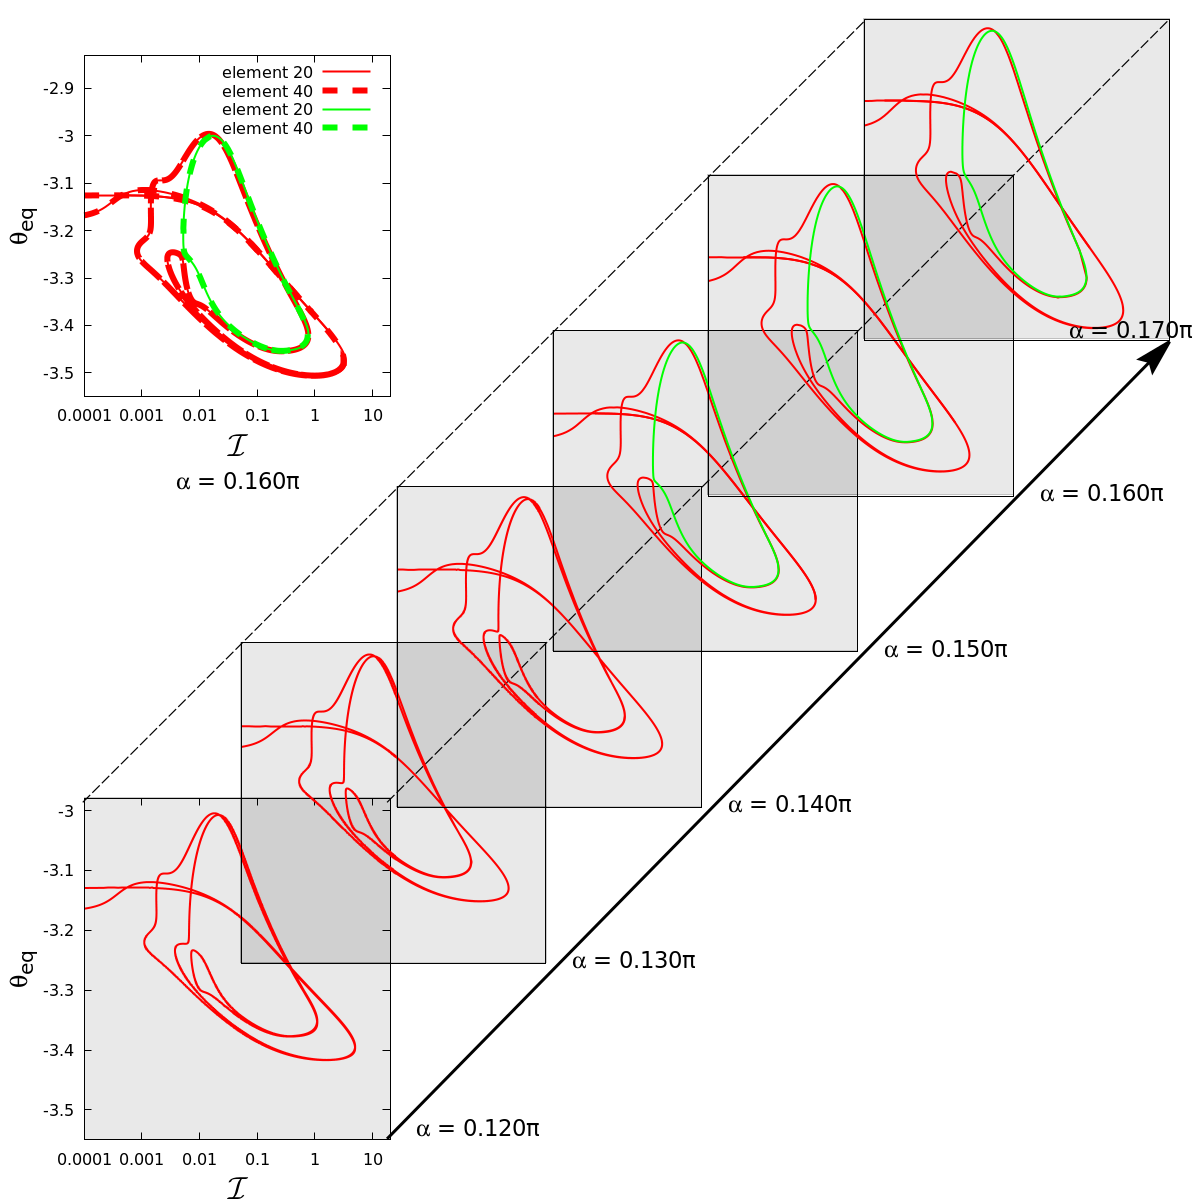
\includegraphics[scale=0.166]{plot/elastic_beam_I_theta_q_0.452_alpha_restart1.png}
	\end{minipage}
	\begin{minipage}{\linewidth}
		\centering
		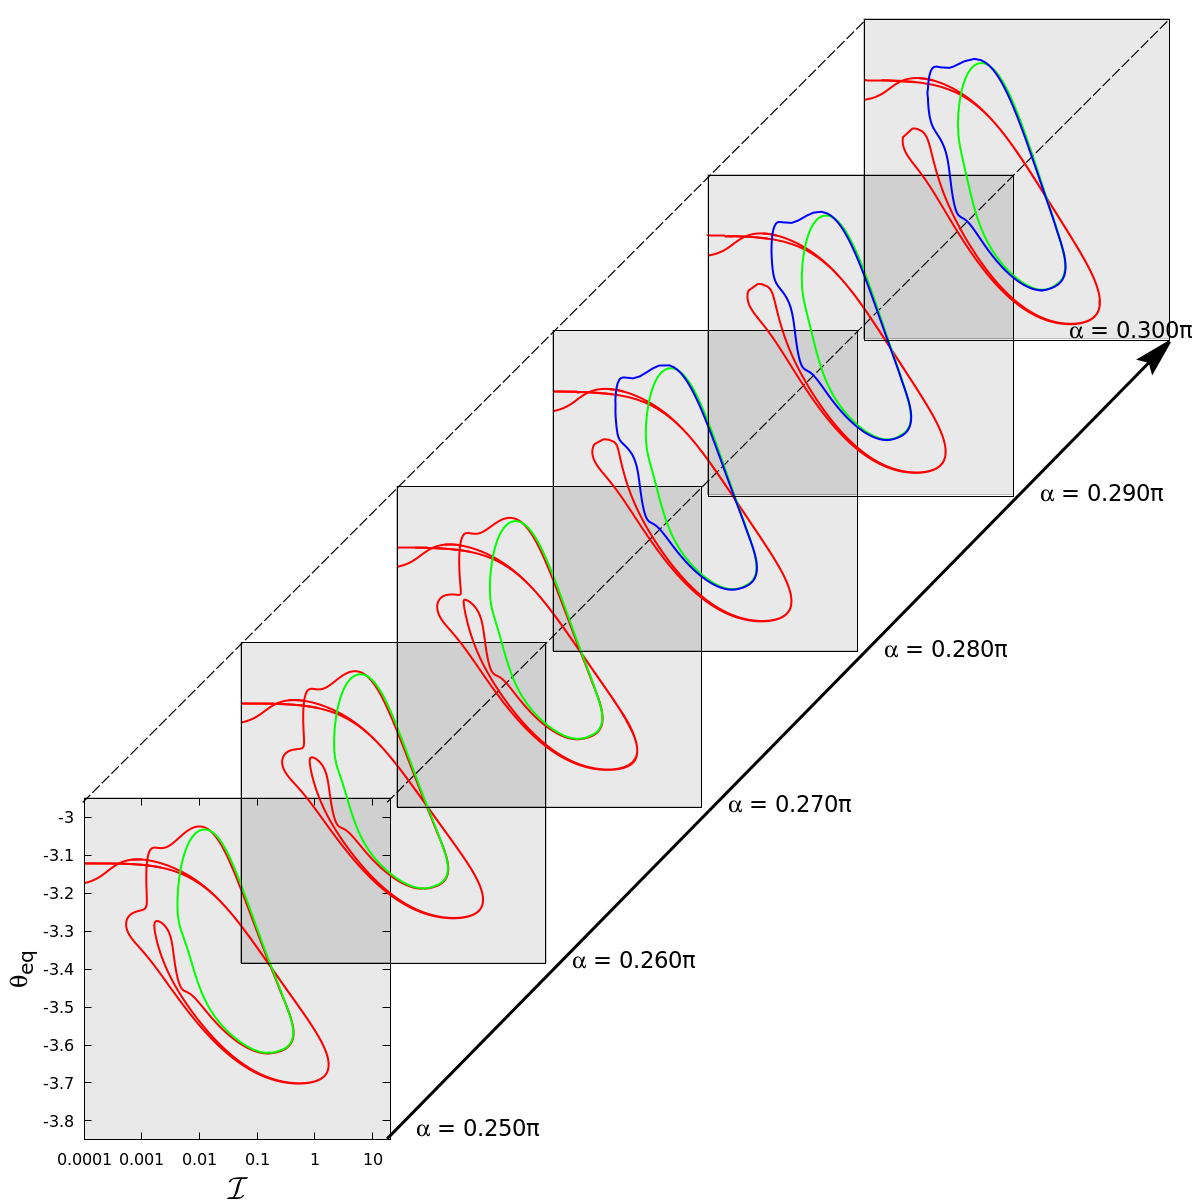
\includegraphics[scale=0.166]{plot/elastic_beam_I_theta_q_0.452_alpha_restart2.png}
	\end{minipage}
	\begin{minipage}{\linewidth}
		\centering
		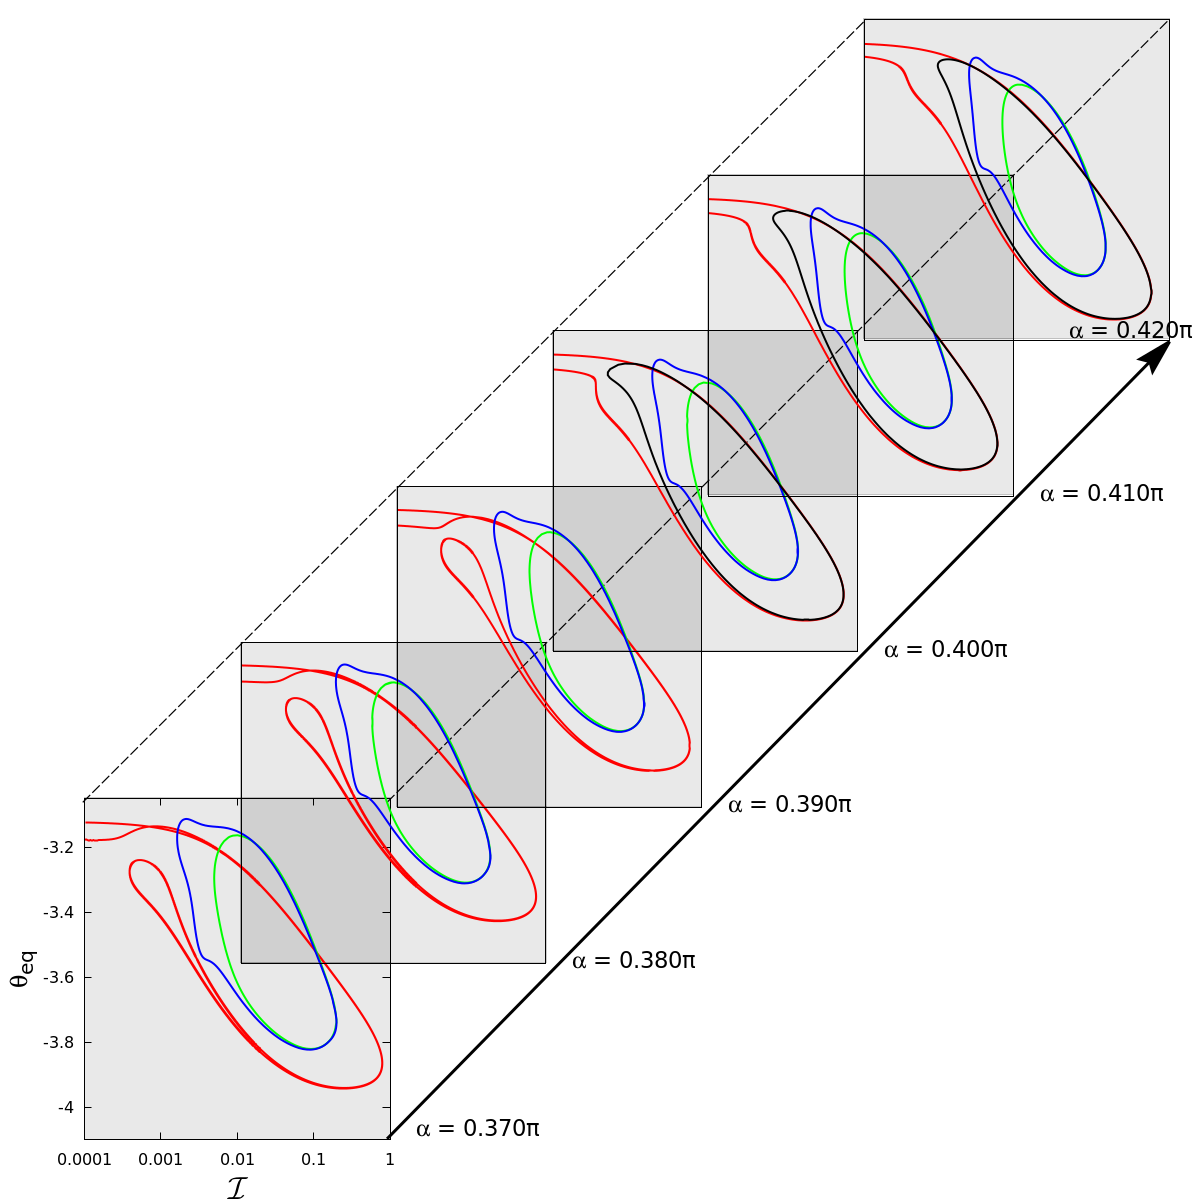
\includegraphics[scale=0.166]{plot/elastic_beam_I_theta_q_0.452_alpha_restart3.png}
	\end{minipage}
	\caption{A sequence of logarithmic plots presents the steady orientation $\theta_{eq}$ against the FSI coefficient $\mathcal{I}$ for shape parameters $q = 0.452$ with varying $\alpha$. The top-left subplot shows the convergence test with doubled elements, and the scale of the axes is consistent across all subplots.}
	\label{fig:11}
\end{figure}
In Figure \ref{fig:11}, there are three bifurcations as $\alpha$ varies, and we have selected three sequences to illustrate them. The explanations are generally similar: as $\alpha$ increases, two distinct protrusions gradually approach each other until they meet at a bifurcation point, causing the curve to split and generate a new independent closed loop. Subsequently, as $\alpha$ continues to increase, this new independent closed loop moves away from the previously connected curve. Finally, the curve splits into three inner closed loops (green, blue and black) and an outermost curve (red) that still connects to the two points at $\mathcal{I} = 0$. Note that after $\alpha=0.4\pi$, the four curves (three inner closed loops and one outermost curve) are independent with each other.

As $q$ increases, causing the short arm to shorten, not only the curve becomes more complex, but additional types of deformation also emerge. Since no significant deformation is observed on the short arm, deformations can be classified by the number of humps appearing on the long arm. In total, four types of deformations are identified within this system, as presented in Table \ref{Table:1}.
\begin{table}[!h]
    \setlength{\belowcaptionskip}{0.8cm}
    \caption{The four types of deformations are categorised by the number of humps appearing on the long arm of the particle.} 
    \label{Table:1}
    \renewcommand\arraystretch{1.5}
    \resizebox{\textwidth}{!}{
    \begin{tabular}{|>{\centering\arraybackslash}m{0.25\textwidth} >{\centering\arraybackslash}m{0.25\textwidth} >{\centering\arraybackslash}m{0.25\textwidth} >{\centering\arraybackslash}m{0.25\textwidth}|}
        \hline
        \hspace{0.8cm}one hump  & \hspace{-0.3cm}two humps& \hspace{-1cm}three humps & \hspace{-1.8cm}four humps \\
        \hline
        \multicolumn{4}{|c|}{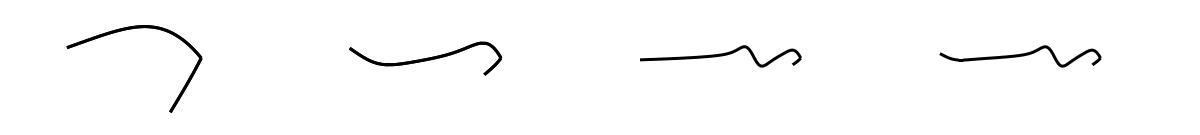
\includegraphics[width=\linewidth]{plot/geometry3.png}} \\
        \hline
    \end{tabular}}
\end{table}

 Similarly to the Roggeveen and Stone's $q-\alpha$ plot in Figure \ref{fig:19}, we aim to determine the boundary of the region where fixed points exist for the elastic particle case. To achieve this, we first plot the  steady orientation $\theta_{eq}$ against the opening angle $\alpha$, as shown in Figure \ref{fig:13}. 
\begin{figure}[!h]
	\begin{center}
		% specify width as 80% of the width of the text on the page
		% we can also specify a width in centimetres, e.g. [width=8cm]
		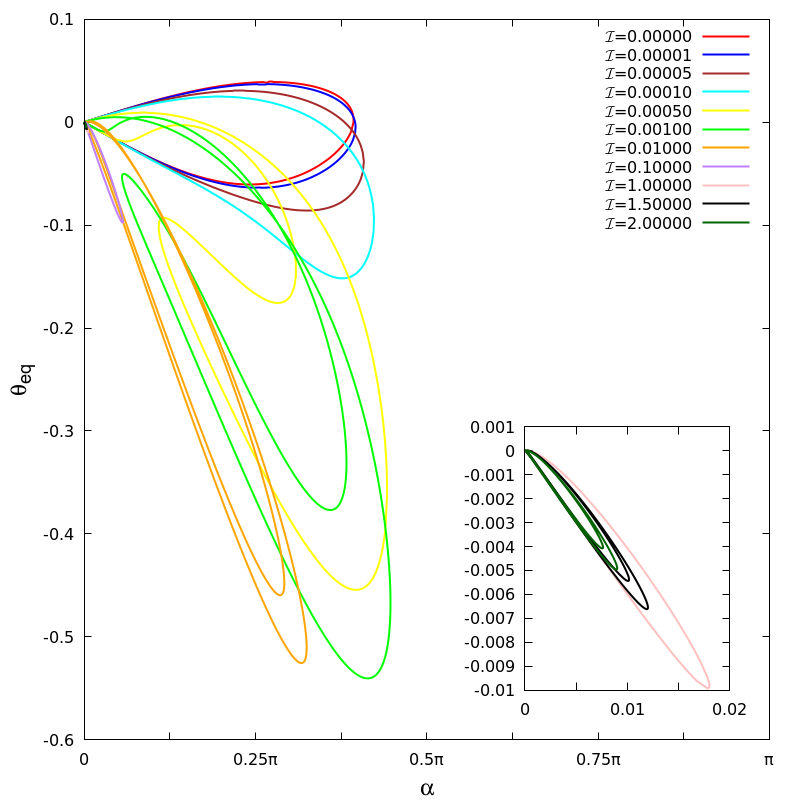
\includegraphics[width=0.75\textwidth]{plot/elastic_beam_alpha_theta_eq_q_0.400.png}
		\caption{The steady orientation $\theta_{eq}$ is plotted against  the opening angle $\alpha$ for the particle with $q = 0.4$. The bottom-right subplot shows the figures of $\mathcal{I}=1.0, 1.5, 2.0$ at a smaller scale.}
    \label{fig:13}
	\end{center}
	%	\setlength{\abovecaptionskip}{-0.5 cm}
\end{figure}
In Figure \ref{fig:13}, as $\mathcal{I}$ increases, $\alpha_{max}$ initially rises and then rapidly decreases. We observe that every curve for different values of $\mathcal{I}$ forms a closed loop. Therefore, by tracing $\alpha_{max}$ for various $\mathcal{I}$, we can determine the boundary of the fixed points region.
\begin{figure}[!h]
	\begin{center}
		% specify width as 80% of the width of the text on the page
		% we can also specify a width in centimetres, e.g. [width=8cm]
		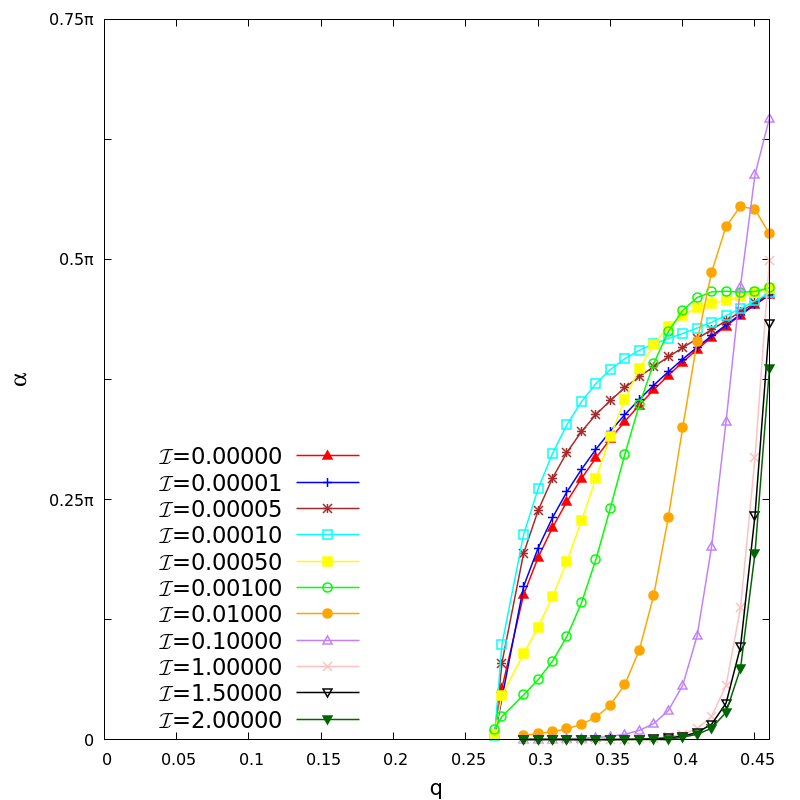
\includegraphics[width=0.75\textwidth]{plot/elastic_beam_general.png}
		\caption{This plot shows the boundary of the fixed points region for different FSI coefficient $\mathcal{I}$.}
    \label{fig:14}
	\end{center}
	%	\setlength{\abovecaptionskip}{-0.5 cm}
\end{figure}
Figure \ref{fig:14} shows the boundary we concern for different FSI coefficient $\mathcal{I}$. The red line represents the boundary for $\mathcal{I}=0$, which aligns with the results from Roggeveen and Stone's paper \cite{roggeveen2022motion}. Generally, as $\mathcal{I}$ increases, the region initially expands and then contracts. We can analyse this plot alongside Figure \ref{fig:13}. Focusing on a vertical line at $q = 0.4$, we observe that as $\mathcal{I}$ increases within the range $[0, 0.001]$ (from red to green), the boundary expands, indicating that $\alpha_{max}$ increases in Figure \ref{fig:13}. However, starting from  $\mathcal{I} = 0.01$ (orange), the region begins to shrink, meaning that $\alpha_{max}$ decreases in Figure \ref{fig:13}. It appears that there is a threshold around $\mathcal{I}=0.001$ (green). Before this threshold, as $\mathcal{I}$ increases, $\alpha_{max}$ also increases. After this point, when $\mathcal{I}$ increases, $\alpha_{max}$ decreases rapidly. In addition, we observe that when $\mathcal{I}\geq1$ (pink), the boundary reaches a relatively solid state. As the value of $\mathcal{I}$ increases, it appears that the boundary approaches its limit and changes more slowly.

\begin{figure}[!h]
	\begin{center}
		% specify width as 80% of the width of the text on the page
		% we can also specify a width in centimetres, e.g. [width=8cm]
		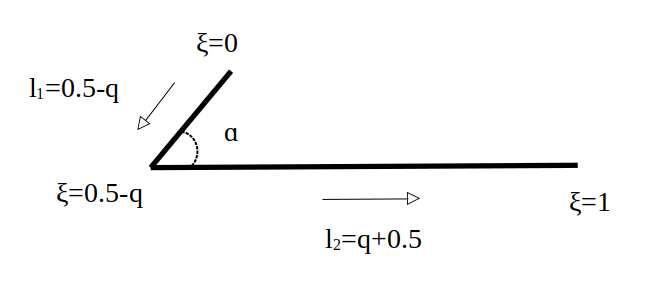
\includegraphics[width=0.7\textwidth]{plot/tensile_boomerang.png}
		\caption{The rigid structure particle ($\mathcal{I}=0$).}
    \label{fig:15}
	\end{center}
	%	\setlength{\abovecaptionskip}{-0.5 cm}
\end{figure}
To understand the mechanism of deformation, we define the tensile stress as 
	\begin{equation}
 \label{eqn:91}
		\sigma(\xi)=\int_0^\xi (\mathbf{f}\cdot\mathbf{t}) \left |\frac{\partial \mathbf{R}}{\partial \xi}\right|\,d\xi,
	\end{equation}
where $\mathbf{t}$ is the unit tangent vector to the surface of the particle. As shown in Figure \ref{fig:15}, we use $\sigma_1$ and $\mathbf{t}_1$ to denote the tensile stress and tangent vector in the short arm, and $\sigma_2$ and $\mathbf{t}_2$ for the long arm. At the hinge point, we have 
	\begin{equation}
 \label{eqn:92}
	\sigma_1(0.5-q)=\mathbf{F}_1\cdot\mathbf{t}_1, 
\end{equation}
	\begin{equation}
 \label{eqn:93}
	\sigma_2(0.5-q)=\mathbf{F}_2\cdot\mathbf{t}_2, 
\end{equation}
where $\mathbf{F}_1$ and $\mathbf{F}_2$ represent the net drag acting on the short arm and long arm, respectively. Then, if $\xi \in [0,0.5-q]$, we have 
	\begin{equation}
 \label{eqn:94}
	\sigma_1(\xi)= \int_0^\xi (\mathbf{f}\cdot\mathbf{t}_1) \left |\frac{\partial \mathbf{R}}{\partial \xi}\right|\,d\xi.
\end{equation}
If $\xi \in [0.5-q,1]$, we have
	\begin{equation}
		\label{eqn:95}
	\begin{aligned}
	\sigma_2(\xi)&= \int_0^\xi (\mathbf{f}\cdot\mathbf{t}_2) \left |\frac{\partial \mathbf{R}}{\partial \xi}\right|\,d\xi\\
	&=\int_0^{0.5-q} (\mathbf{f}\cdot\mathbf{t}_2) \left |\frac{\partial \mathbf{R}}{\partial \xi}\right|\,d\xi+\int_{0.5-q}^\xi (\mathbf{f}\cdot\mathbf{t}_2) \left |\frac{\partial \mathbf{R}}{\partial \xi}\right|\,d\xi\\
	&=\mathbf{F}_1\cdot\mathbf{t}_2+\int_{0.5-q}^\xi (\mathbf{f}\cdot\mathbf{t}_2) \left |\frac{\partial \mathbf{R}}{\partial \xi}\right|\,d\xi.
\end{aligned}
\end{equation}
Since we are investigating the equilibrium state, the components of the two net drag forces in the $\mathbf{t}_2$ direction must also be balanced. Hence, we have 
\begin{equation}
	\label{eqn:96}
	\mathbf{F}_1\cdot\mathbf{t}_2=-\mathbf{F}_2\cdot\mathbf{t}_2.
\end{equation}
Now, substituting \eqref{eqn:96} into the last step of \eqref{eqn:95}, we obtain 
\begin{equation}
	\begin{aligned}
	\label{eqn:97}
\sigma_2(\xi)&=-\mathbf{F}_2\cdot\mathbf{t}_2+\int_{0.5-q}^\xi (\mathbf{f}\cdot\mathbf{t}_2) \left |\frac{\partial \mathbf{R}}{\partial \xi}\right|\,d\xi\\
&=-\sigma_2(0.5-q)+\int_{0.5-q}^\xi (\mathbf{f}\cdot\mathbf{t}_2) \left |\frac{\partial \mathbf{R}}{\partial \xi}\right|\,d\xi.
\end{aligned}
\end{equation}
Therefore, we have 
\begin{equation}
	\sigma(\xi)=\left\{
	\begin{aligned}
		\label{eqn:98}
		&\int_0^\xi (\mathbf{f}\cdot\mathbf{t}_1) \left |\frac{\partial \mathbf{R}}{\partial \xi}\right|\,d\xi,\quad \xi\in[0,0.5-q];\\
		&-\mathbf{F}_2\cdot\mathbf{t}_2+\int_{0.5-q}^\xi (\mathbf{f}\cdot\mathbf{t}_2) \left |\frac{\partial \mathbf{R}}{\partial \xi}\right|\,d\xi, \quad \xi\in[0.5-q,1].
	\end{aligned}\right.
\end{equation}
\begin{figure}[!h]
	\centering
	\subfigure[$q=0.35,\alpha=0.125\pi$]{
		\begin{minipage}[b]{0.31\textwidth}
			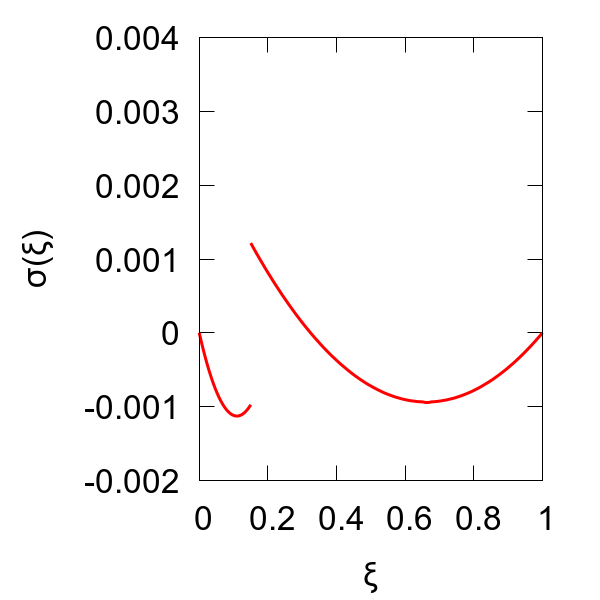
\includegraphics[width=1\textwidth]{plot/sigma_q_0.35_alpha_0.125pi.png} 
		\end{minipage}
		\label{fig:16.a}
	}
	\subfigure[$q=0.40,\alpha=0.125\pi$]{
		\begin{minipage}[b]{0.31\textwidth}
			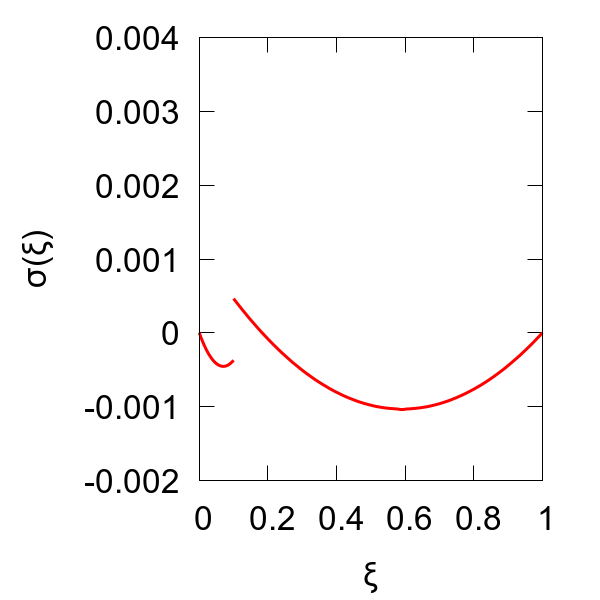
\includegraphics[width=1\textwidth]{plot/sigma_q_0.4_alpha_0.125pi.png}
		\end{minipage}
		\label{fig:16.b}
	}
    \subfigure[$q=0.45,\alpha=0.125\pi$]{
    	\begin{minipage}[b]{0.31\textwidth}
    		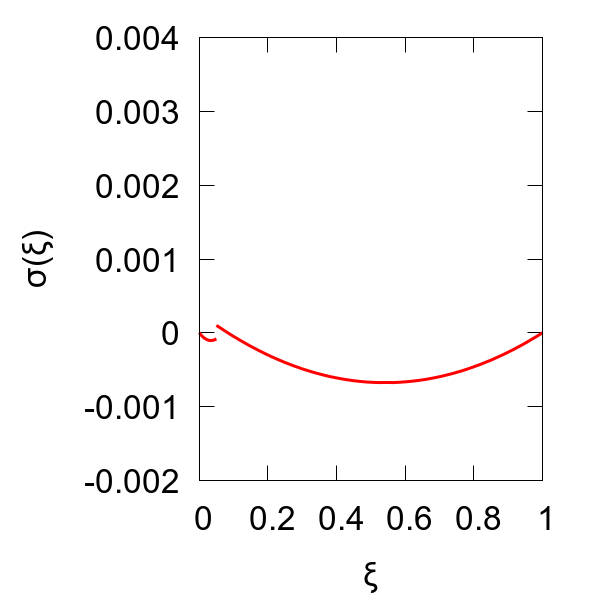
\includegraphics[width=1\textwidth]{plot/sigma_q_0.45_alpha_0.125pi.png}
    	\end{minipage}
    	\label{fig:16.c}
    }
	\\ 
	\subfigure[$q=0.35,\alpha=0.25\pi$]{
		\begin{minipage}[b]{0.31\textwidth}
				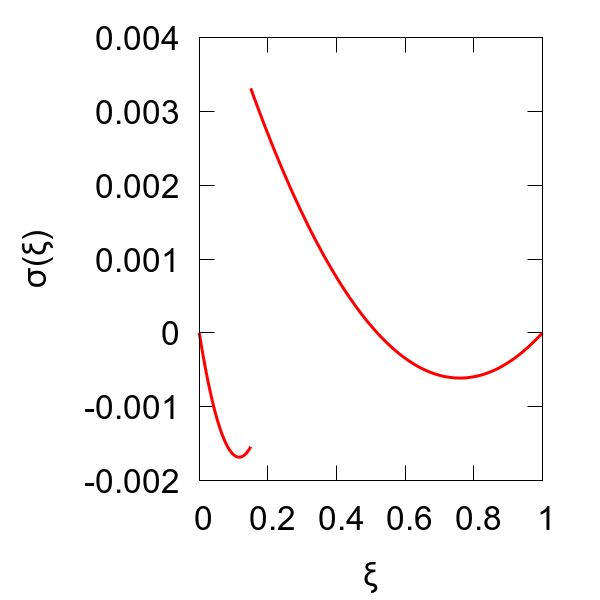
\includegraphics[width=1\textwidth]{plot/sigma_q_0.35_alpha_0.25pi.png} 
		\end{minipage}
		\label{fig:16.d}
	}
	\subfigure[$q=0.40,\alpha=0.25\pi$]{
		\begin{minipage}[b]{0.31\textwidth}
			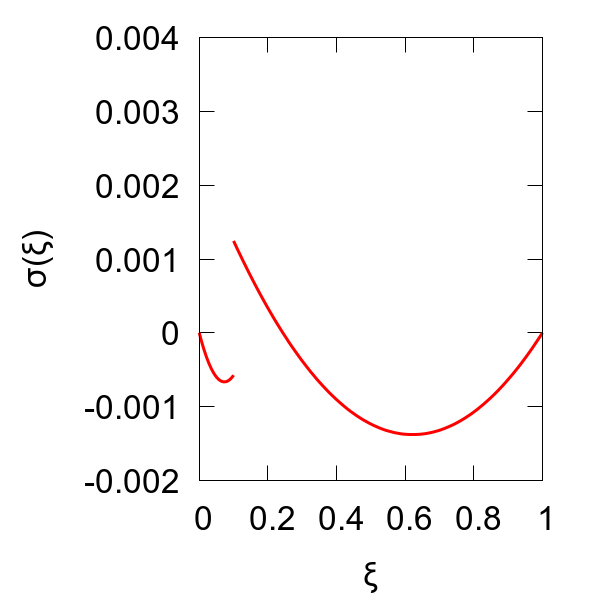
\includegraphics[width=1\textwidth]{plot/sigma_q_0.4_alpha_0.25pi.png}
		\end{minipage}
		\label{fig:16.e}
	}
    \subfigure[$q=0.45,\alpha=0.25\pi$]{
    	\begin{minipage}[b]{0.31\textwidth}
    		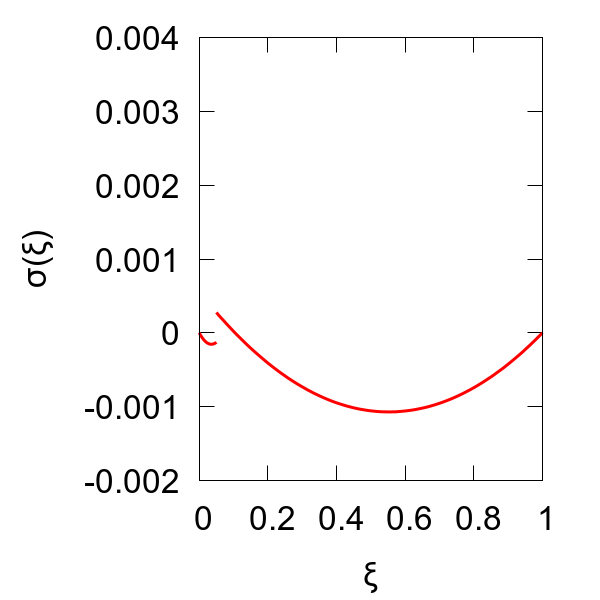
\includegraphics[width=1\textwidth]{plot/sigma_q_0.45_alpha_0.25pi.png}
    	\end{minipage}
    	\label{fig:16.f}
    }
	\caption{Tensile stress for different shape parameters ($\mathcal{I}=0$).}
	\label{fig:16}
\end{figure}
Figure \ref{fig:16} presents the six results of the tensile stress for different shape parameters when $\mathcal{I}=0$. When $\xi=0$ or $\xi=1$, $\sigma=0$, which is consistent with the fact that no force acts on the free ends. Each plot shows a jump discontinuity at the hinge point. It can be observed that the tensile stress at this point is non-zero and has opposite signs on either side, indicating a complex mechanical relationship at the hinge. The curves illustrate the tensile stress experienced by the rigid particle under fluid forces, indicating a tendency for deformation if it were made of elastic material. 


\chapter{Conclusions}
In this report, we investigate the dynamics of an elastic particle in shear flow at a low Reynolds number, with particular focus on the particle's equilibrium state. We continue to use the slender boomerang shape from Roggeveen and Stone \cite{roggeveen2022motion} as the initial configuration  for inextensible elastic particles, because it can qualitatively represent the behaviour of more complex bodies. We apply slender body theory to evaluate the traction exerted by the fluid and integrate it as net drag, then derive the net torque to satisfy the drag-free and torque-free conditions. In solid mechanics, we use Kirchhoff-Love Beam theory to establish the governing equation for the elastic beam. Following the idea of fluid-solid interaction, we define the fluid-solid interaction coefficient $\mathcal{I}$ using the relationship between the non-dimensional fluid and non-dimensional solid traction to measure the degree or strength of interaction between the fluid and the solid within the system. When the FSI coefficient $\mathcal{I}=0$, the particle transforms into a rigid material, consistent with the findings of Roggeveen and Stone \cite{roggeveen2022motion}. Thus, we validate the numerical results for $\mathcal{I}=0$, demonstrating the reliability of our model. We also show that particle's deformation is time-independent and derive the specific expression for the translational vector $\mathbf{r}_b$. Similar to the rigid case, it also drifts uniformly with a fixed orientation. Subsequently, we use the finite element method combined with the Newton method to solve the differential equations numerically, programming the algorithm using \texttt{oomph-lib}.

We visualise the numerical data to depict the particle's deformation at various values of the FSI coefficient. In total, four distinct types of deformation are identified, which we categorise based on the number of humps appearing on the long arm of the particle. We also present some graphs of the steady orientation $\theta_{eq}$ against the FSI coefficient $\mathcal{I}$, revealing some interesting bifurcations along the curve. The general description is that as the opening angle $\alpha$ increases, two distinct protrusions gradually approach each other until they meet at a bifurcation point, causing the curve to split and generate a new independent curve. Subsequently, as $\alpha$ continues to increase, this new independent closed loop moves away from the previously connected curve. We also observe that these bifurcations only occur when the aspect ratio $q$ is relatively large (basically greater than $0.38$), which means that the short arm of the particle is comparatively small. To determine which initial shapes of the particle can reach the equilibrium state, we present a $q-\alpha$ plot to illustrate the layout of the region where fixed orientations occur at different values of the FSI coefficient $\mathcal{I}$. Then, to figure out the mechanics of the deformation, we define the tensile stress for the rigid case to observe the deformation tendency exerted by the fluid on the particle.

Generally, we consider the hydrodynamic interactions between the two arms to be negligible. However, when in close proximity to the hinge point, or when the opening angle $\alpha$ is too small, the interactions between the arms cannot be ignored at sufficiently small scales. We also consider only the case of a single elastic particle in shear flow, without accounting for interactions with other particles, because the movement of a particle is typically governed by its interaction with the background flow rather than with other particles. From the numerical results, we find that as the aspect ratio $q$ increases, indicating that the short arm is shorter, the curve of the steady orientation against the FSI coefficient becomes increasingly complex, exhibiting numerous twists along the curve. Meanwhile, the deformation of the particle also becomes more intricate. We also know that the opening angle $\alpha$ is related to the occurrence of bifurcations. Therefore, they reflect that the initial shapes of the particle are crucial in this system.



\chapter{Future plan}
Until now, we have investigated the dynamics of an elastic particle in shear flow at a low Reynolds number, which serves as a warm-up study for our more ambitious project. Briefly, our ambitious aim is to explore the sedimentation of an elastic disk in Stokes flow, which will be based on the results completed by Vaquero-Stainer et al. \cite{vaquero2024u}. It is well established that a flat circular disk sediments in Stokes flow at a low Reynolds number with constant horizontal drift, maintaining a fixed orientation \cite{brenner1963stokes}. Vaquero-Stainer et al. extended this work by introducing a U-shaped disk (created by the isometric deformation of a circular disk onto the surface of a circular cylinder), demonstrating that with a specific initial orientation, the U-shaped disk retains its inclination and follows a perfectly spiral trajectory during sedimentation. Given that the shape of the rigid disk can be varied from flat to U-shaped by adjusting its curvature, they also investigate the influence of curvature on the different sedimentation behaviours observed. We aim to transition the disk material from rigid to elastic by incorporating the fluid-solid interaction (FSI) coefficient. However, given the substantial computational time required even for the rigid case, directly studying the elastic case is impractical. That is why we start from a warm-up project involving a two-dimensional problem to pave the way for more complex analyses.

It is also known that the straight rod exhibits motion similar to that of a flat circular disk in Stokes flow, with constant horizontal drift and fixed orientation \cite{brenner1963stokes}. We are considering a sequence of shapes, from a flat circular disk to a fibre. In the middle of the sequence, excluding the ends, there is a series of ellipses with a constant major axis equal to the circle's diameter, while the minor axis gradually decreases. Intuitively, the U-shaped disk represents a general configuration when a flexible, flat circular disk sediments in Stokes flow, which is beneficial for studying the elastic case. For a straight fibre, its 'U-shape' will degenerate and remain as a fibre. However, for the 'U-shape' formed by a series of ellipses, the specific motion remains unknown. Given that the computational process for a circular disk is too costly, it may be more efficient to evaluate the cases of ellipses. We believe that starting with an ellipse with a very small minor axis is a promising approach. Although this is a three-dimensional problem, its shape closely resembles that of a fibre, suggesting that its motion and analysis may be similar to the two-dimensional fibre problem.

In addition, we believe it is sensible in the next step to simulate the buckling process of an initially straight elastic fibre in shear flow at a low Reynolds number. It is a similar buckling process to that of the elastic circular disk, but at a lower cost. We have found that, apart from the boomerang-shaped particle with a hinge point, some rigid asymmetric U-shaped particles also exhibit steady solutions, which could inspire further research into the buckling process for elastic materials. In low Reynolds number flows, shapes with high symmetry often exhibit relatively simple dynamical characteristics. Some studies demonstrate that in simple shear flows, a rigidly curved slender body with a plane of reflective symmetry can display chaotic trajectories \cite{thorp2019motion} and persistent cross-streamline drift \cite{wang2012flipping}, depending on the particle's shape and initial orientation. This conclusion partially supports our results, which show that the asymmetric U-shaped rigid fibre also has steady solutions.


%\begin{thebibliography}{999}
%\bibitem{ANO} A.N.~Other, ....
%\end{thebibliography}
\bibliography{references}

% Comment the following THREE lines if you do NOT have an Appendix
%\appendix
%\chapter{A Long Proof}


% If you need more than one appendix, then just use another \chapter command
%\chapter{Yet Another Appendix}

\end{document}
